\chapter{Results and discussion}\label{chap:Results&Disc}
In this chapter the results and methods from laboratory experiments are presented and discussed.

\section{PFAS sorption in biochar-water batch tests}
In \cref{fig:sorption_isotherms}, the sorption isotherms are presented for PFPeA, PFHxA, PFHpA, PFOA, PFNA and PFDA to CWC, ULS and DSL. The points generated from the batch tests were fitted using the Freundlich model (\cref{eq:FreundlichLinear}). For all compounds, the sorption isotherm for ULS is visibly higher than DSL, followed by CWC. The Freundlich sorption coefficients ($log~K_F$), linearity coefficients ($n_F$) and correlation coefficients ($r^2$) are presented in \cref{tab:summary_stats_single}. Somewhat unexpectedly, sorption is strongest for the two sludge chars. Possible mechanisms for the strong sorption will be discussed in this section. 

Due to the pioneering research on sewage sludge biochars as sorbents for PFAS in this thesis, literature partitioning coefficients for PFCAs of other sewage sludge biochars are non-existent (is that correct?). However, a comparison can be made between the $log~K_F$s found in this thesis and for commercially-produced activated carbons (AC) from other studies. The sorption coefficients are equivalent or higher compared to literature values for $log~K_F$ of PFOA to AC: 5.60 \citep{Kupryianchyk2016a}, 4.45 \citep{hansen2010sorption}, and 4.74-5.42 \citep{silvani2019can}. This is promising for the potential to replace non-renewable AC with waste based biochars for environmental remediation in the field and wastewater treatment. 

\begin{figure}[tb]
    \centering
    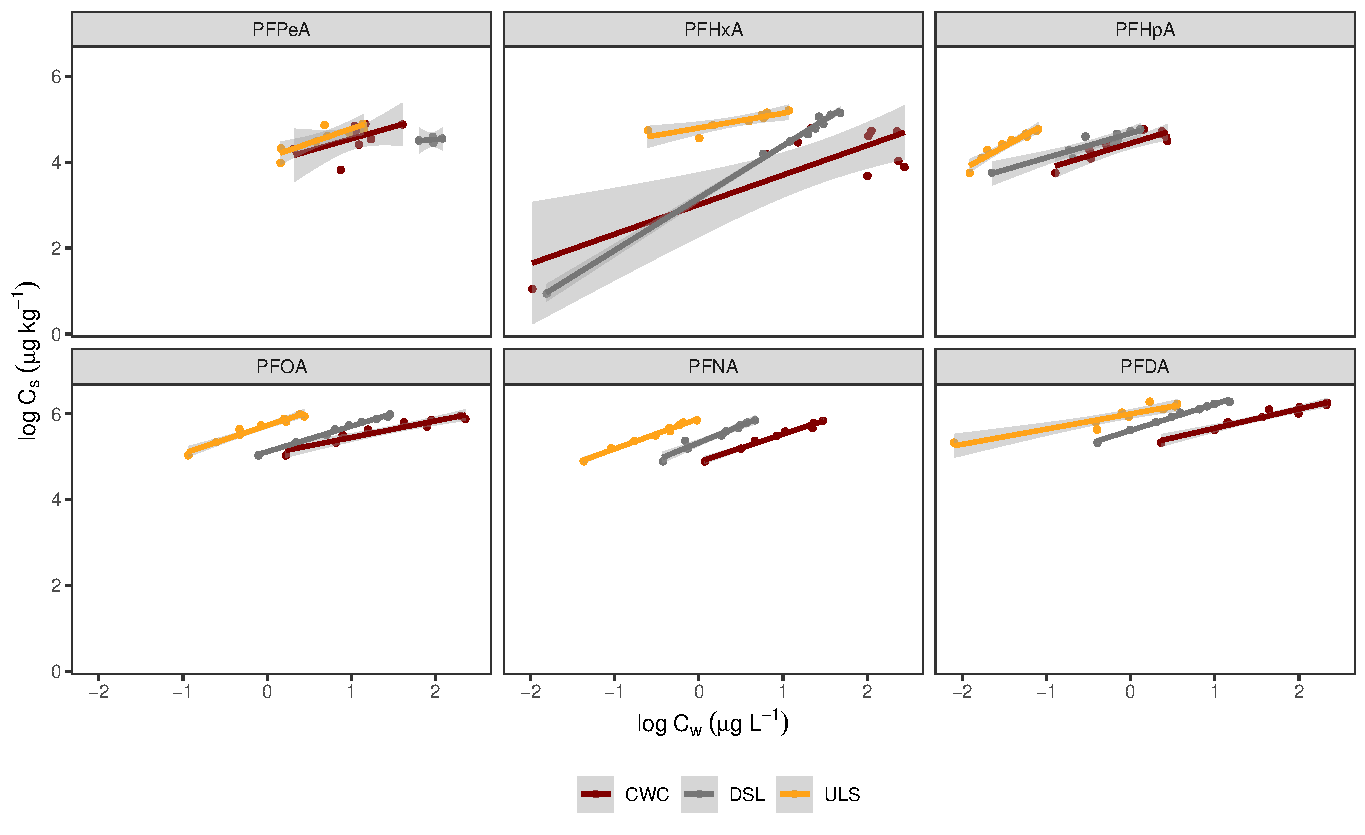
\includegraphics[width=\textwidth]{R/figs/Sorption_isotherms_single_BC.pdf}
    \caption{Freundlich isotherms of TCs in batch tests with three different biochars. Lines are obtained by linear regression.}
    \label{fig:sorption_isotherms}
\end{figure}

\begin{table}
\caption{Freundlich sorption parameters of single TC isotherms in CWC, ULS and DSL (n=9). The error is presented as standard error. All $K_F$ data are in units of $\mathrm{(\mu g/kg)/(\mu g/L)^{n_F}}$.}
\centering
\adjustbox{max width=\textwidth}{%
\begin{threeparttable}
\label{tab:summary_stats_single}
\begin{tabular}{lllllllllllll} \toprule
PFCA & \multicolumn{4}{c}{ULS} & \multicolumn{4}{c}{DSL} & \multicolumn{4}{c}{CWC} \\ \cmidrule(l){2-5} \cmidrule(l){6-9} \cmidrule(l){10-13}
 & $log~K_{F,BC}$ & $n_{F,BC}$ & $r^2$ & $p$ & $log~K_{F,BC}$ & $n_{F,BC}$ & $r^2$ & $p$ & $log~K_{F,BC}$ & $n_{F,BC}$ & $r^2$ & $p$ \\ \midrule
PFPeA & 4.10 ± 0.13 & 0.67 ± 0.16 & 0.74 & ** & 4.25 ± 0.74 & 0.14 ± 0.38 & 0.06 & $>$0.05 & 3.98 ± 0.36 & 0.56 ± 0.33 & 0.30 & $>$0.05 \\
PFHxA & 4.80 ± 0.06 & 0.34 ± 0.09 & 0.72 & ** & 3.30 ± 0.15 & 1.11 ± 0.11 & 0.93 & *** & 4.59 ± 0.50 & -0.14 ± 0.26 & 0.04 & $>$0.05 \\
PFHpA & 5.98 ± 0.17 & 1.08 ± 0.11 & 0.93 & *** & 4.67 ± 0.06 & 0.57 ± 0.09 & 0.86 & *** & 4.44 ± 0.05 & 0.59 ± 0.11 & 0.80 & ** \\
PFOA & 5.73 ± 0.02 & 0.65 ± 0.05 & 0.95 & *** & 5.12 ± 0.02 & 0.60 ± 0.02 & 0.99 & *** & 5.06 ± 0.08 & 0.39 ± 0.05 & 0.90 & *** \\
PFNA & 5.89 ± 0.02 & 0.71 ± 0.03 & 0.99 & *** & 5.33 ± 0.03 & 0.80 ± 0.07 & 0.94 & *** & 4.88 ± 0.04 & 0.65 ± 0.04 & 0.98 & *** \\
PFDA & 6.00 ± 0.04 & 0.35 ± 0.05 & 0.86 & *** & 5.61 ± 0.02 & 0.61 ± 0.02 & 0.99 & *** & 5.22 ± 0.07 & 0.45 ± 0.04 & 0.94 & *** \\ \bottomrule
\end{tabular}
\begin{tablenotes}
\item Significant codes: *** $\sim$ 0.001, ** $\sim$ 0.01,  
\end{tablenotes}
\end{threeparttable}}
\end{table}

\cite{du2014adsorption}: electr and hydry balance 

\subsection{Effect of PFAS chain length}
\cref{fig:sorption_isotherms_all} shows sorption isotherms for the single-compound batch tests for CWC, ULS and DSL. The Freundlich coefficients for ULS increased in the order, PFPeA $<$ PFHxA $<$ PFOA $<$ PFHpA $<$ PFNA $<$ PFDA, ranging from $log~K_F$ = 4.10-6.00 (\cref{tab:summary_stats_single}). All regressions were significant (p$<$0.01). The Freundlich coefficients for DSL increased in the order, PFHxA $<$ PFPeA $<$ PFHpA $<$ PFOA $<$ PFNA $<$ PFDA, ranging from $log~K_F$ = 3.16-5.61. All regressions were significant (p$<$0.001) except for the PFPeA isotherm which only consisted of four points (SP7-10) due to higher analyzed filtrate concentrations than what was spiked for SP1-6 (attributed to analytical uncertainty or imprecision/contamination during laboratory work) (\cref{fig:DSL_isotherm}). The Freundlich coefficients for CWC increased in the order, PFPeA $<$ PFHpA $<$ PFHxA $<$ PFNA $<$ PFOA $<$ PFDA, ranging from $log~K_F$ = 3.01-5.22. All regressions were significant (p$<$0.01) except for PFPeA and PFHxA despite nine points used in the regressions. Changes in $log~K_F$ with chain length can be visualized in \cref{subfig:chainlength}. 

A statistically significant relationship between $log~K_F$ and CF\textsubscript{2} chain length was found for all three biochars (p$<$0.05, \cref{fig:chain_length_n}), which is in accordance with previous studies \citep{Sorengard2019,higgins2006sorption,ahmed2020per}. There was a difference of 1.2-1.9 $log~K_F$ units between the longest and the shortest PFCA chain (PFDA and PFPeA). For every CF\textsubscript{2} moiety, hydrophobic interactions between condensed aromatic structures in the biochar matrix increases, contributing to stronger sorption. Several mechanisms can be used to explain why perfluorinated carboxylic acids increase in hydrophobicity with increasing chain length. 1) Due to high molecular surface of the perfluorinated tail, a high cavity formation energy is needed to dissolve the compounds in water, and therefore they tend to be pushed towards water extremities, such as a biochar surface. Therefore, dissolution becomes increasingly energetically demanding with increasing chain length \citep{sigmund2022sorption}. 2) the perfluorinated chain with CF\textsubscript{2} moieties is capable of the least van der Waals interactions per molecular surface area compared to CH\textsubscript{2} which results in the least interactions between water molecules when in the water cavity. This is why PFASs are both oil- and water repellent. 

\begin{figure*}[t!]
    \centering
    \begin{subfigure}[t]{0.5\textwidth}
        \centering
        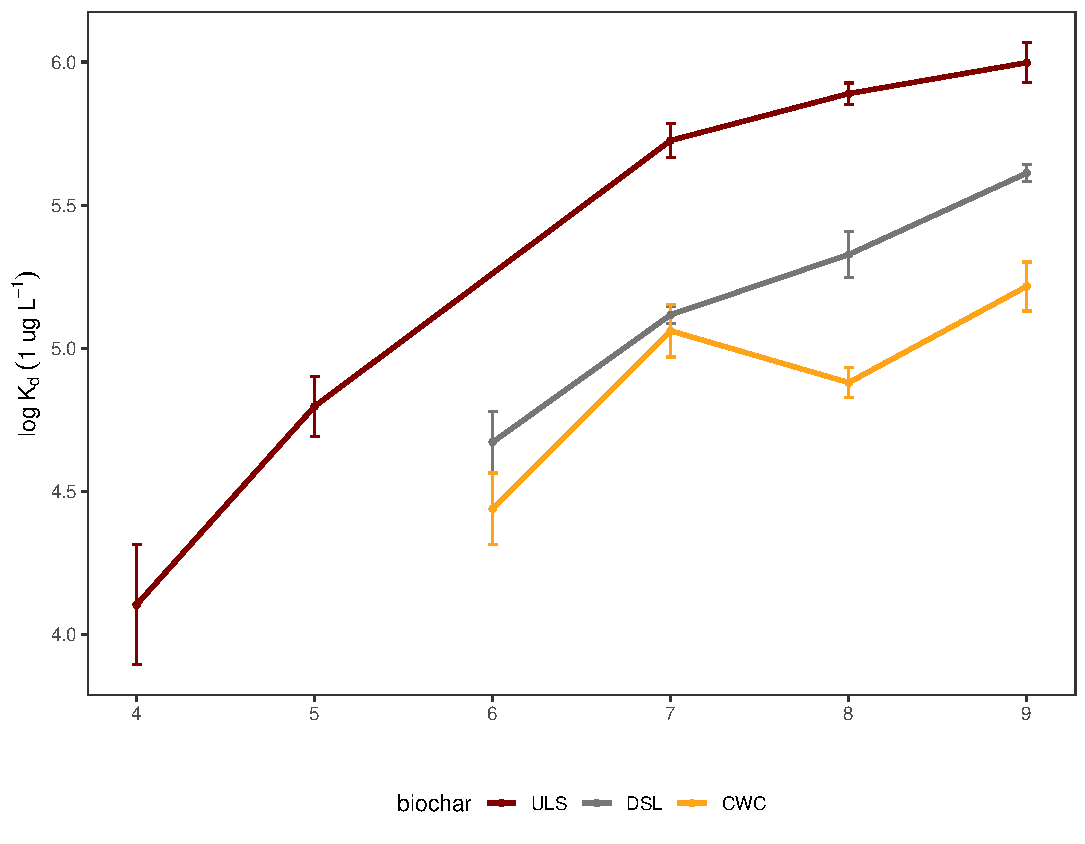
\includegraphics[height=6cm]{R/figs/Kd_1ugL_plot.pdf}
        \caption{}
        \label{subfig:chainlength}
    \end{subfigure}%
    ~ 
    \begin{subfigure}[t]{0.5\textwidth}
        \centering
        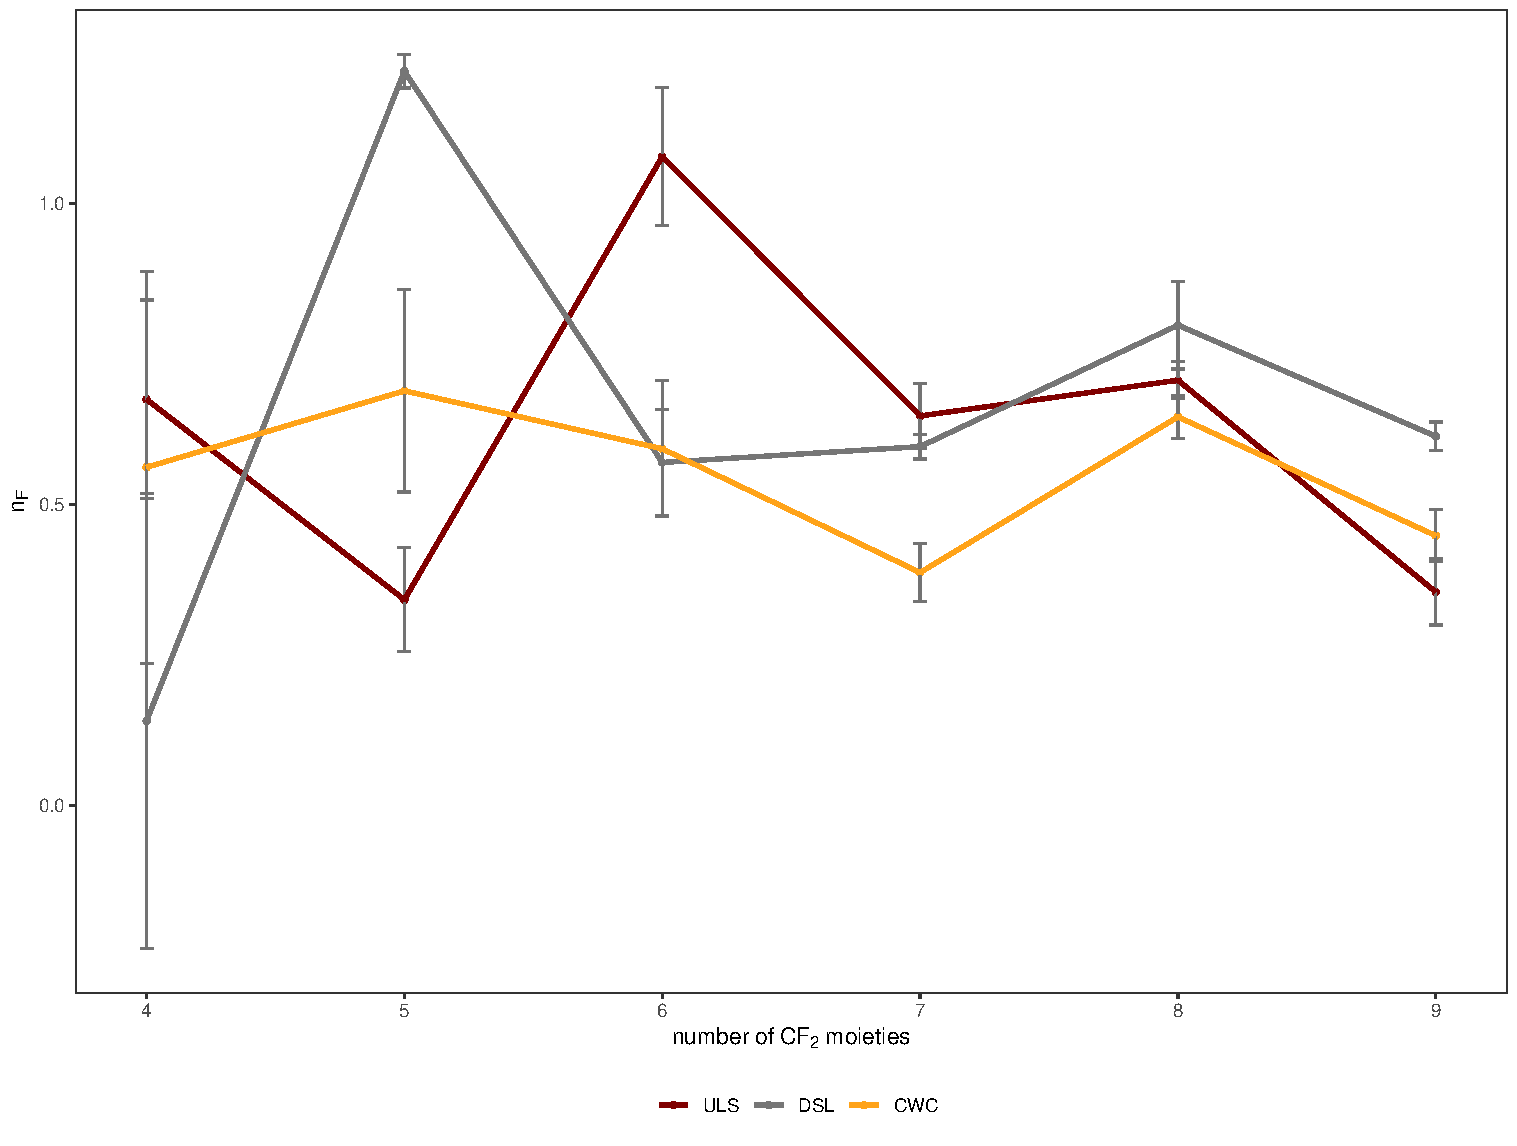
\includegraphics[height=6cm]{R/figs/n_KF.pdf}
        \caption{}
        \label{subfig:n}
    \end{subfigure}
    \label{fig:chain_length_n}
    \caption{Relationship between \textbf{(a)} $log~K_F$ and chain length. Error bars are the propagated error of log KF and n. UPDATE REGRESSION COEFFICIENTS, IN NOTEBOOK. Linear regression coefficients for $log~K_F$ dependency on chain length for ULS: $r^2$ = 0.72, $p$ = 0.013, DSL: $r^2$ = 0.72, $p$ = 0.034, CWC: $r^2$ = 0.82, $p$ = 0.032, and \textbf{(b)} $n_F$ and $CF_2$ chain length. Error bars are the standard error of $log~K_F$ for each chain length and biochar isotherm.}
\end{figure*}

\begin{figure}
    \centering
        \begin{subfigure}[t]{\linewidth}
            \centering
            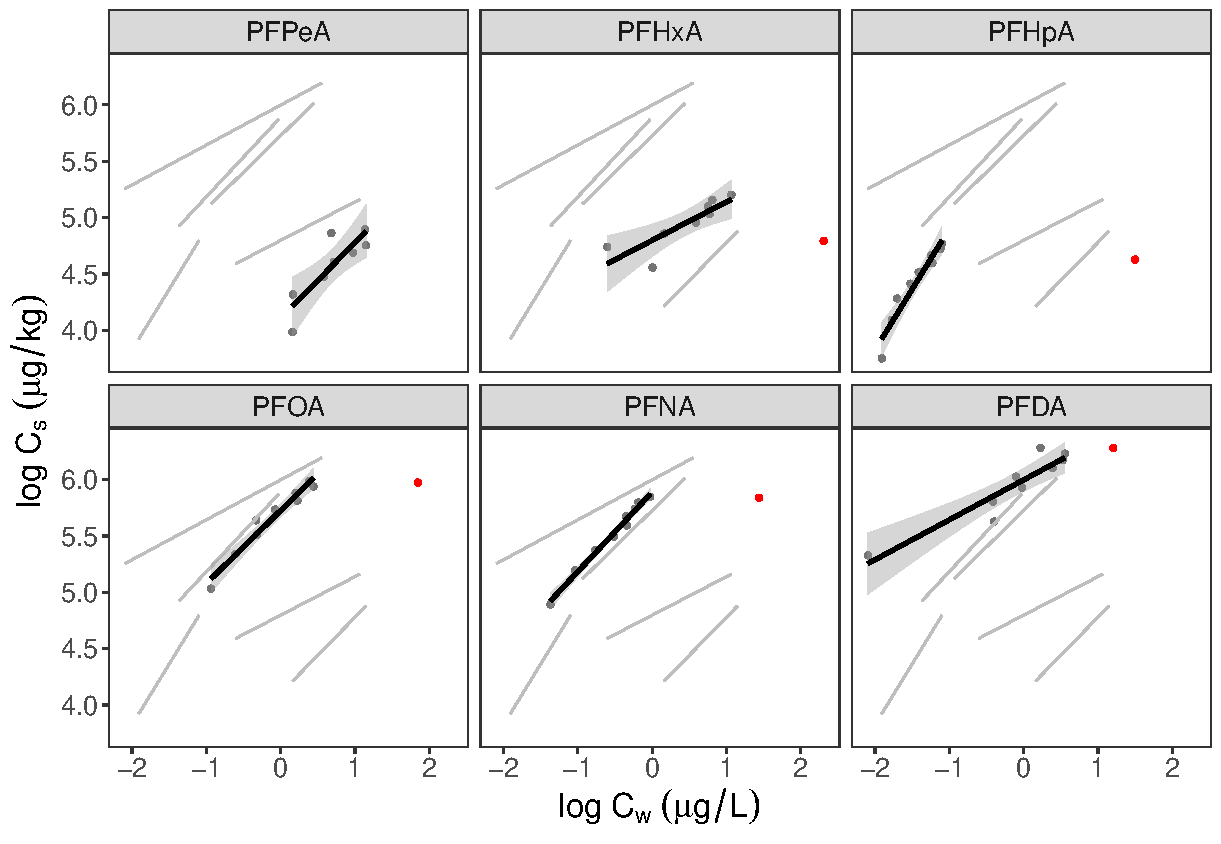
\includegraphics[width=0.8\textwidth]{R/figs/ULS_facet_isotherm.pdf}
            \subcaption{ULS isotherms}
            \label{fig:ULS_isotherm}
        \end{subfigure}
        \begin{subfigure}[]{\linewidth}
            \centering
            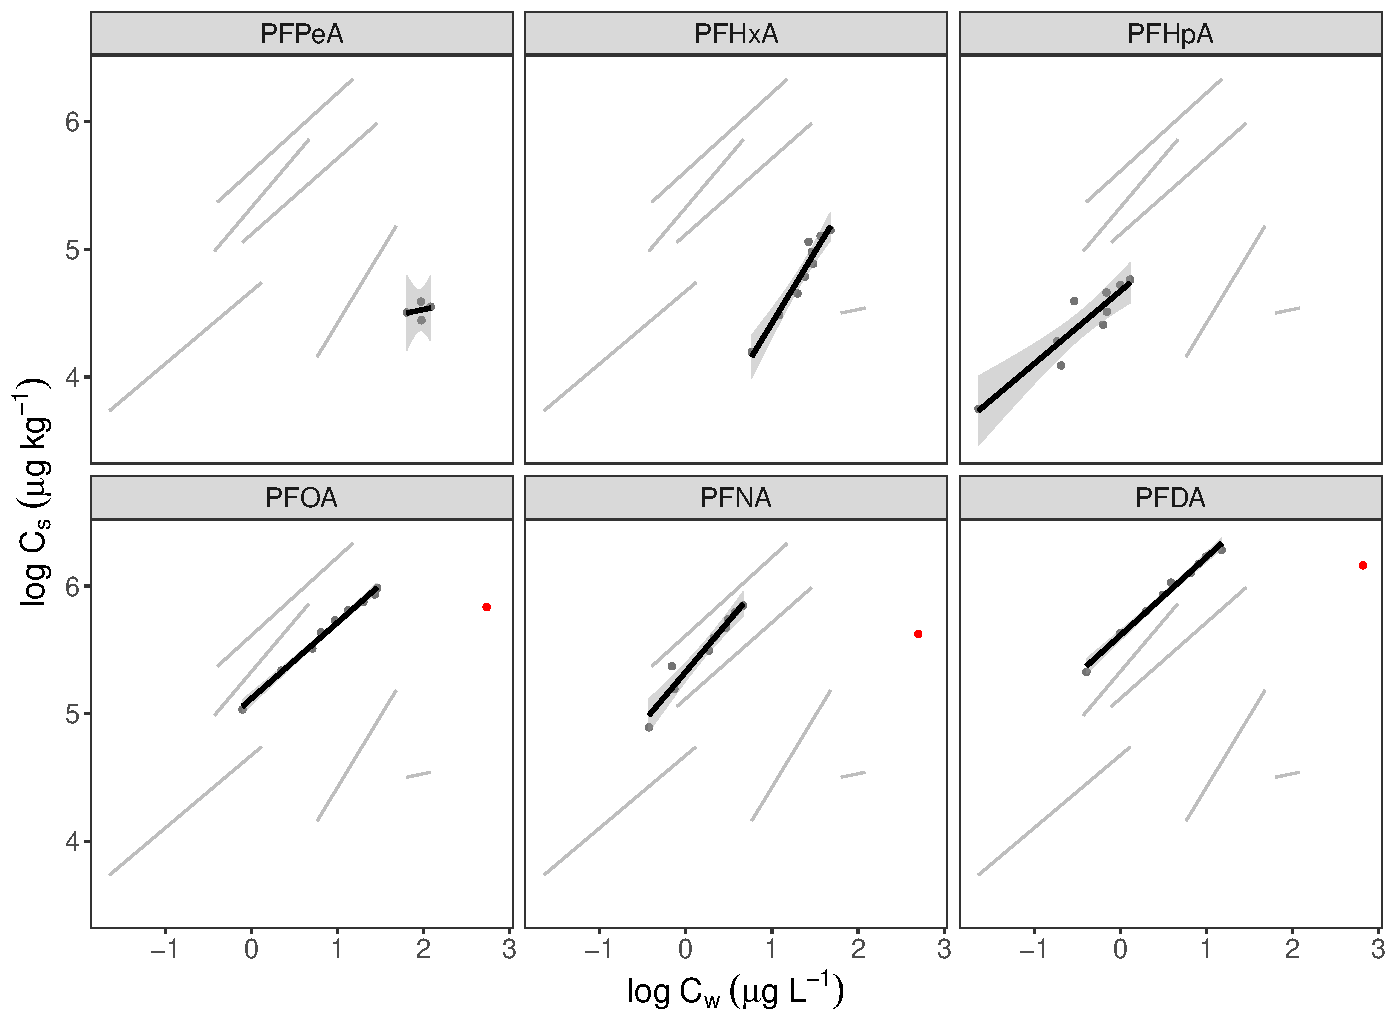
\includegraphics[width=0.8\textwidth]{R/figs/DSL_facet_isotherm.pdf}
            \subcaption{DSL isotherms}
            \label{fig:DSL_isotherm}
        \end{subfigure}   
\end{figure}
\begin{figure}[t]\ContinuedFloat
        \begin{subfigure}[]{\linewidth}
            \centering
            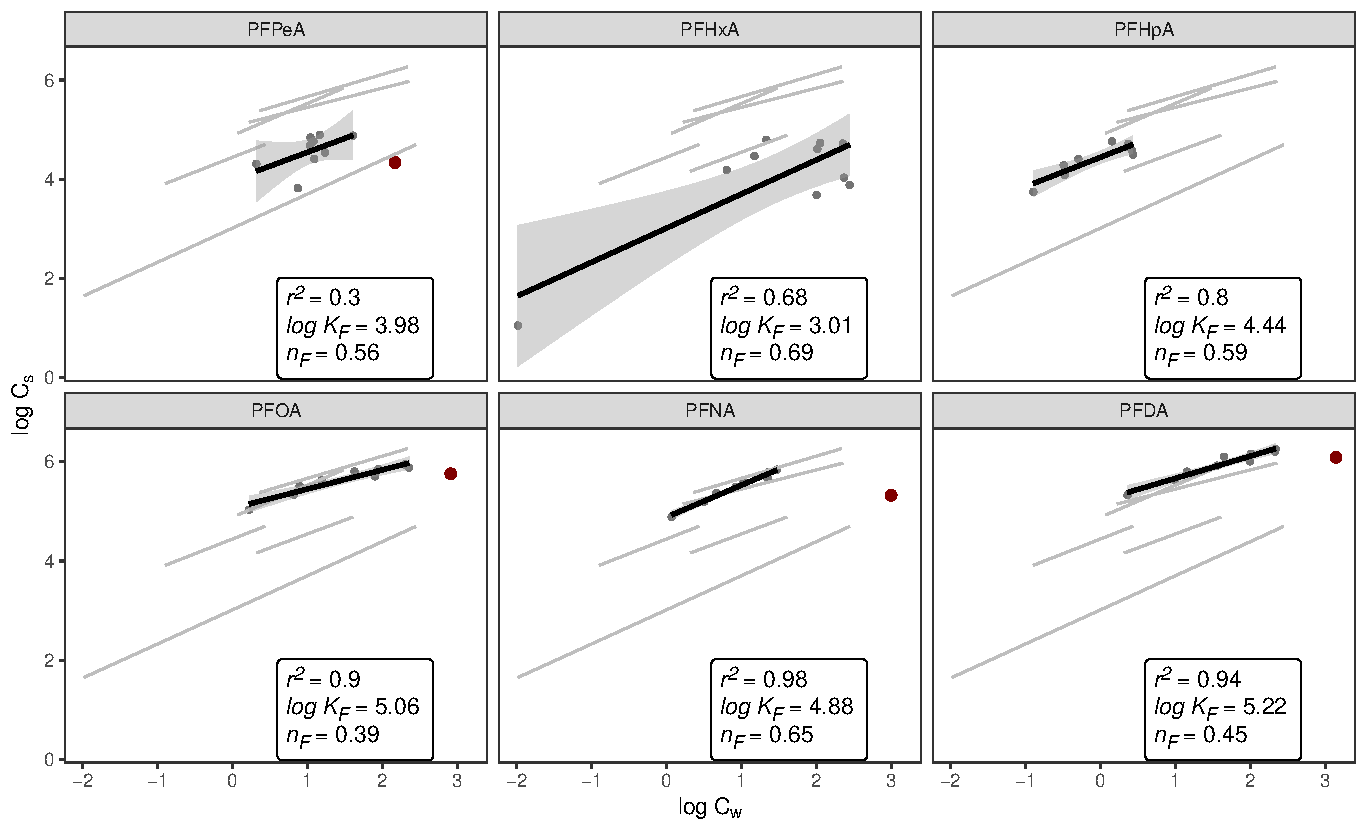
\includegraphics[width=0.8\textwidth]{R/figs/CWC_facet_isotherm.pdf}
            \subcaption{CWC isotherms}
            \label{fig:CWC_isotherm}
        \end{subfigure}
        \caption{Single-compound Freundlich sorption isotherms of PFPeA, PFHxA, PFHpA, PFOA, PFNA and PFDA. Lines are obtained by linear regression.}
        \label{fig:sorption_isotherms_all}
\end{figure}

\subsection{Effect of PFAS functional group} 
The charged and polar head of PFCAs give these compound classes unique sorptive properties because the polar head can engage simultaneously in electrostatic bonding with surface functional groups or bridging cations within the biochar matrix (ash rich in cations) \citep{zhang2013sorption,sigmund2022sorption}. In this study, highest sorption were seen for ULS and DSL with the lowest \% C (\cref{tab:SAPV}), which is in contrast with previous literature. However, previous PFAS sorption studies have been conducted on biochar from cleaner, wood-based feedstock \citep{Sormo2021}, activated carbon \citep{zhang2021sorption,Kupryianchyk2016b}, soils and sediments \citep{higgins2006sorption}, and raw sewage sludges \citep{zhang2013sorption}. These studies conclude that the importance of electrostatic interaction to sorption comes secondary to the hydrophobic effect. The main reason for this is that the biochar surface is net negatively charged with a high cation exchange capacity (CEC) \citep{Ahmad2014} and may experience electrostatic repulsion of the negatively charged functional group. PFCAs have low $pK_a$s (-1, \citep{goss2008pKa}) due to having strong electron withdrawing fluorine atoms and hence become strong acids. The PFCAs investigated in this study will be negatively charged given the filtrate pH of 7.1-7.4 (\cref{tab:pHcond}). Thus, all TCs experience electrostatic repulsion from the biochar surface which result in the lowest $K_F$-values for the shorter-chain PFCAs (\cref{tab:summary_stats_single}). Electrostatic repulsion is reduced in acid soils where the CEC is reduced and the biochar surfaces become protonated and more neutral. This allows for anion- \textpi bond interaction with biochar \citep{sigmund2022sorption}. 

\cite{zhang2021sorption} found that sorption increased in the order PFBA $<$ PFBS $<$ PFOA $<$ PFOS for granular activated carbon and softwood-derived biochar. The difference between the PFSA and PFCA groups is that PFSAs have one more perfluorinated carbon than PFCAs, which has its terminal carbon bonded as a carboxylate (COO\textsuperscript{-}). If one compares PFHpS with PFOA, which have the same number of $\mathrm{CF_2}$ moieties, the perfluorinated sulfonic acid still sorbs better. Researchers attribute this to 1) difference in molecular size, where the sulfonate moiety is slightly larger than the carboxylate moiety, which results in greater cavity formation energy of PFSAs, and hence in water saturated conditions, the functional group is pushed towards water extremities. In batch shaking experiments this would be the biochar surfaces or tube walls \citep{yin2022insights,sigmund2022sorption}, and 2) because sulfonic acid is a stronger acid than carboxylic acid which results in stronger ionic interaction to positive charges of mineral phases \citep{arvaniti2015review}.

Since sorption increased with chain length onto all three biochars in this study, this suggests that hydrophobic interactions is the dominant sorption mechanism over electrostatic interactions. Therefore, further investigation to explain why the sludge biochars sorb better than CWC will follow. 

\subsection{Effect of sorbent properties}
\subsubsection{Main elements}
Based on feedstock type for the three biochars studied in this thesis, carbon content of the biochars follows the expected trend, CWC \textless ULS \textless DSL with 91.4\%, 29.6\% and 13.5\%, respectively (\cref{tab:SAPV}). Oxygen content was highest for DSL and ULS (61.4 and 57.1 \% respectively) compared to 5.5 \% for CWC. CWC has a low O/C and H/C ratio (\textless 1) whereas ULS and DSL have ratios \textgreater 1. A low H/C and O/C ratio is associated with high degree of aromaticity and few functional groups. This shows that the CWC matrix is dominated by aromatic carbon whereas ULS and DSL are dominated by oxidized carbon resulting in a more hydrophobic surface of the high-C biochar. The proportion of elements other than C, O, H and N contained in the biochar matrices is significantly lower for the clean wood biochar (1.4 \%) compared to the sludge biochars (10.9 and 23.2 \%), containing a greater mixture of other elements. Total elemental composition of the biochars is given in \cref{appSec:elements}. The results from this study is in contrast to literature \citep{Hale2016,Sormo2021,zhang2021sorption} that report that the sorption strength of organic compounds to biochar increases with decreasing biochar O/C and biochar H/C ratios. Thus, the higher sorption onto ULS and DSL cannot be explained by the sorbent composition of main elements alone.

\subsubsection{Ionic composition}
Previous research suggests that calcium content is an important parameter contributing to stronger sorption of anionic organic molecules \citep{higgins2006sorption,sigmund2022sorption}. In this study, PFAS sorption to sludge enhanced with increasing calcium concentration in solution, divalent ions contribute to stronger sorption compared to monovalent ions due to ion bridging between negatively charged PFAS and biochar at low pH \citep{zhang2013sorption,arvaniti2014sorption,arvaniti2015review}. 
\citep{yin2022insights} effects of salinity on sorption, states sorption increases with increasing salinity. 

Do I have data on \% ash for each sorbent?

\begin{figure*}[t!]
    \centering
    \begin{subfigure}[t]{0.5\textwidth}
        \centering
        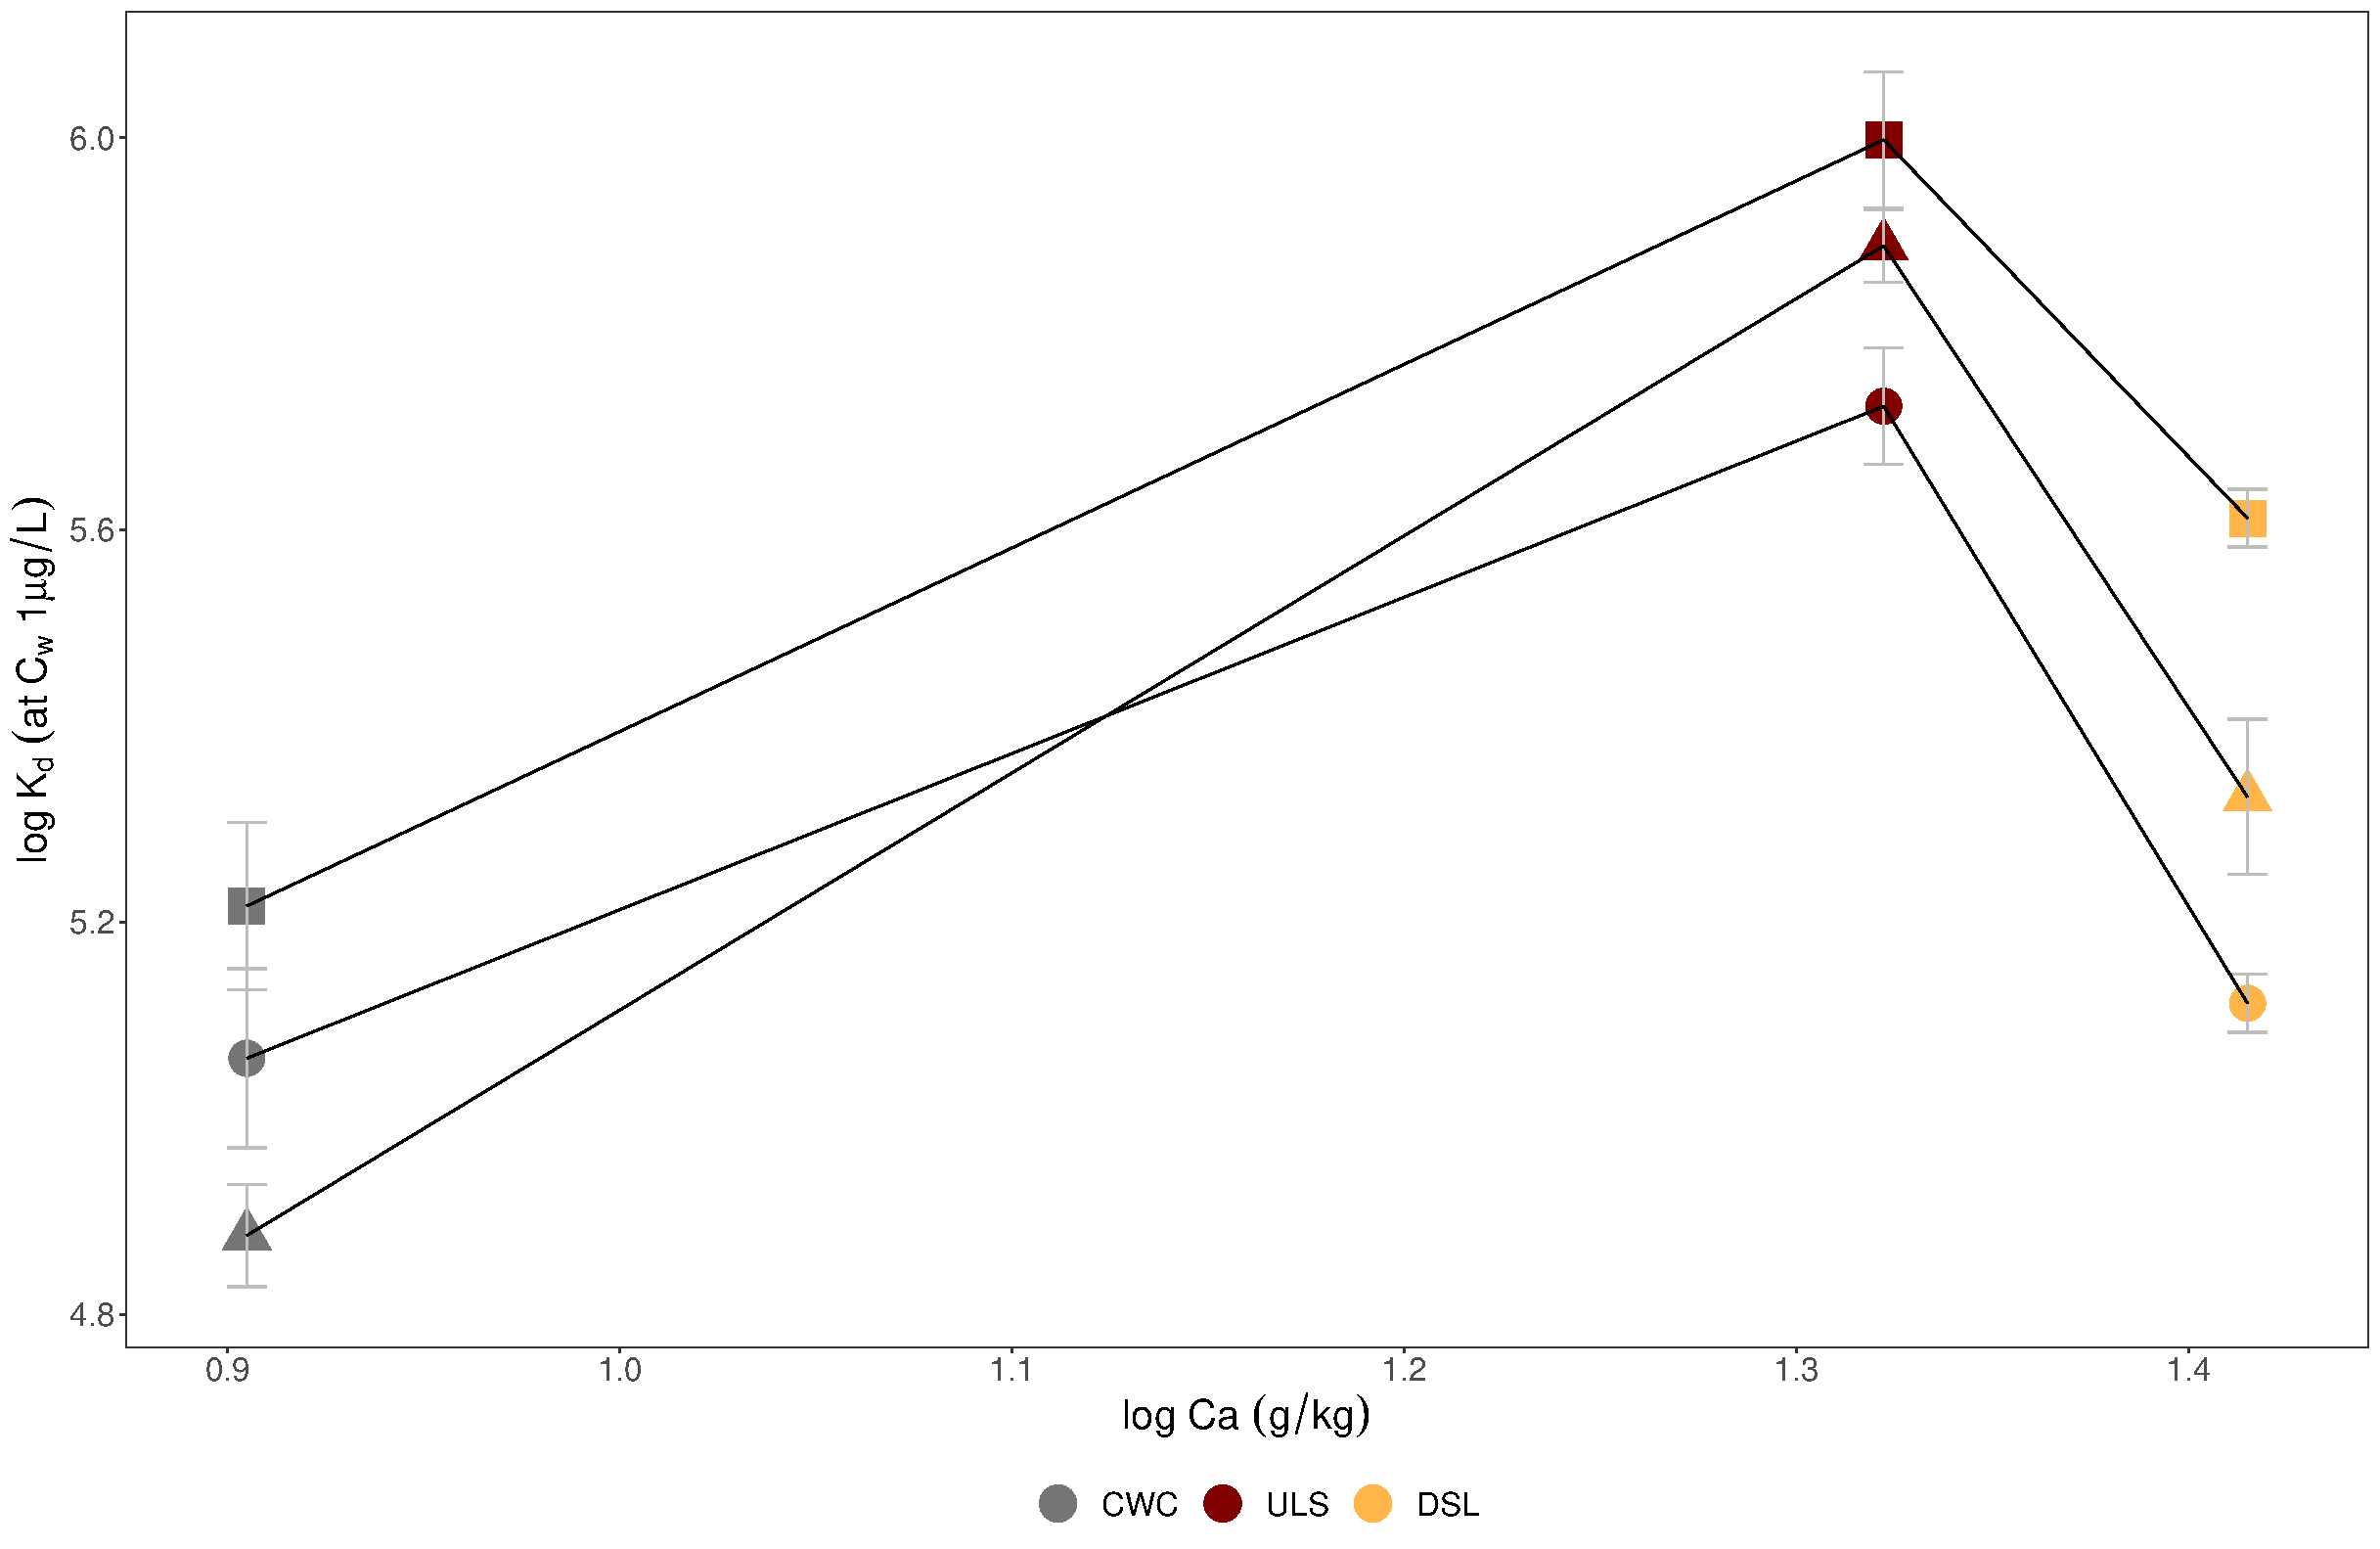
\includegraphics[height=6cm]{R/figs/Kd_1ugL_Ca.pdf}
        \caption{}
        \label{subfig:Ca}
    \end{subfigure}%
    ~ 
    \begin{subfigure}[t]{0.5\textwidth}
        \centering
        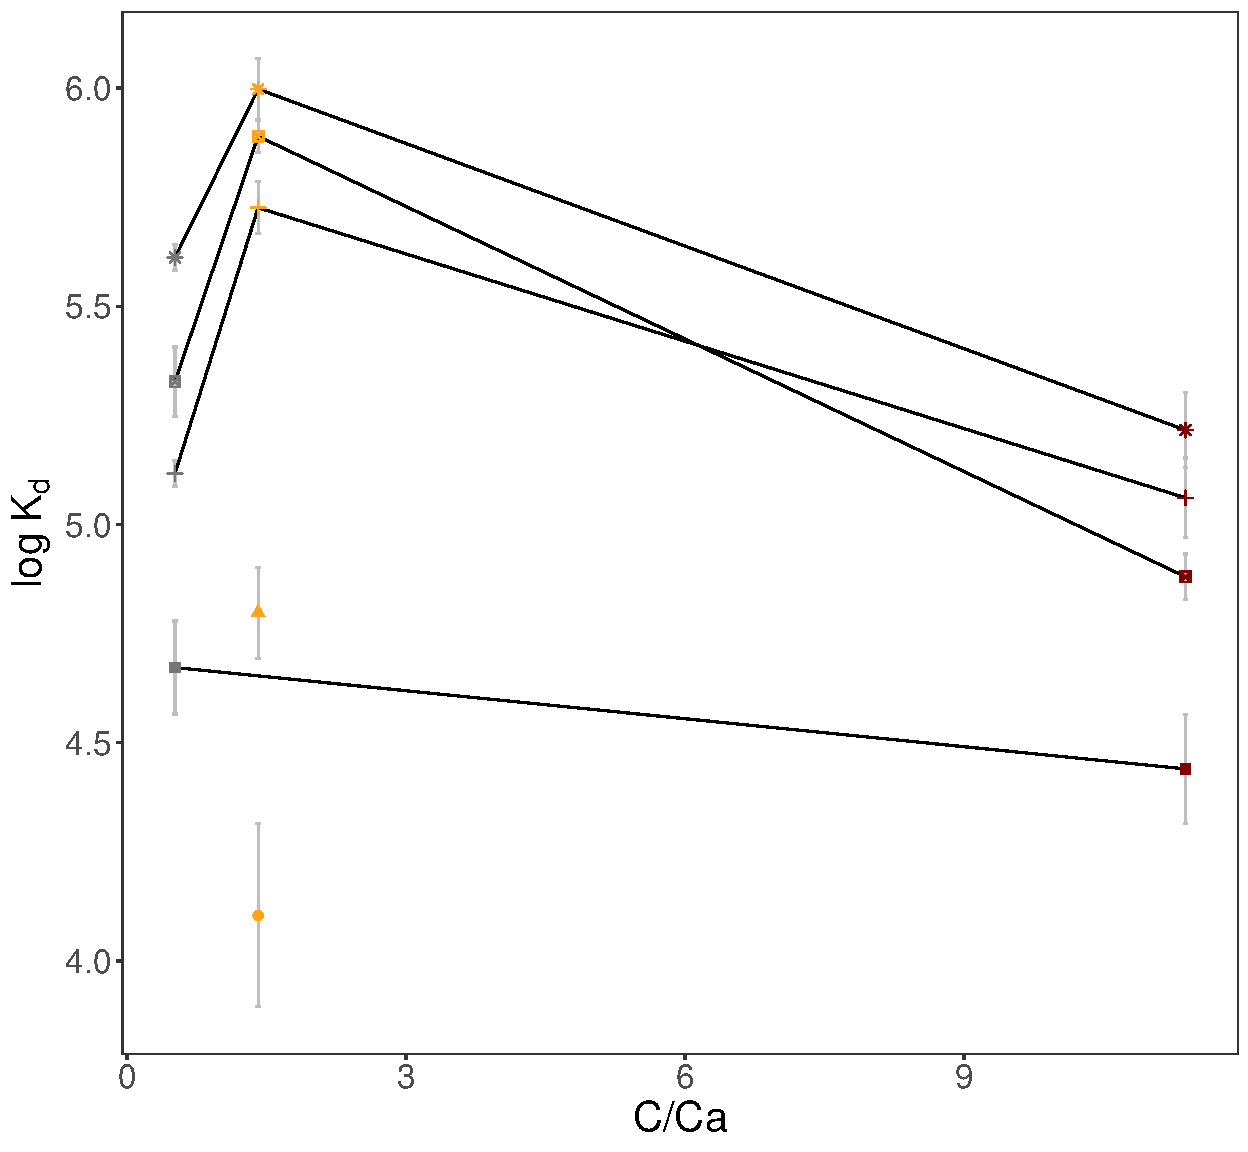
\includegraphics[height=6cm]{R/figs/Kd_1ugL_C_Ca.pdf}
        \caption{}
        \label{subfig:C_Ca}
    \end{subfigure}
    \caption{}
    \begin{subfigure}[t]{0.5\textwidth}
        \centering
        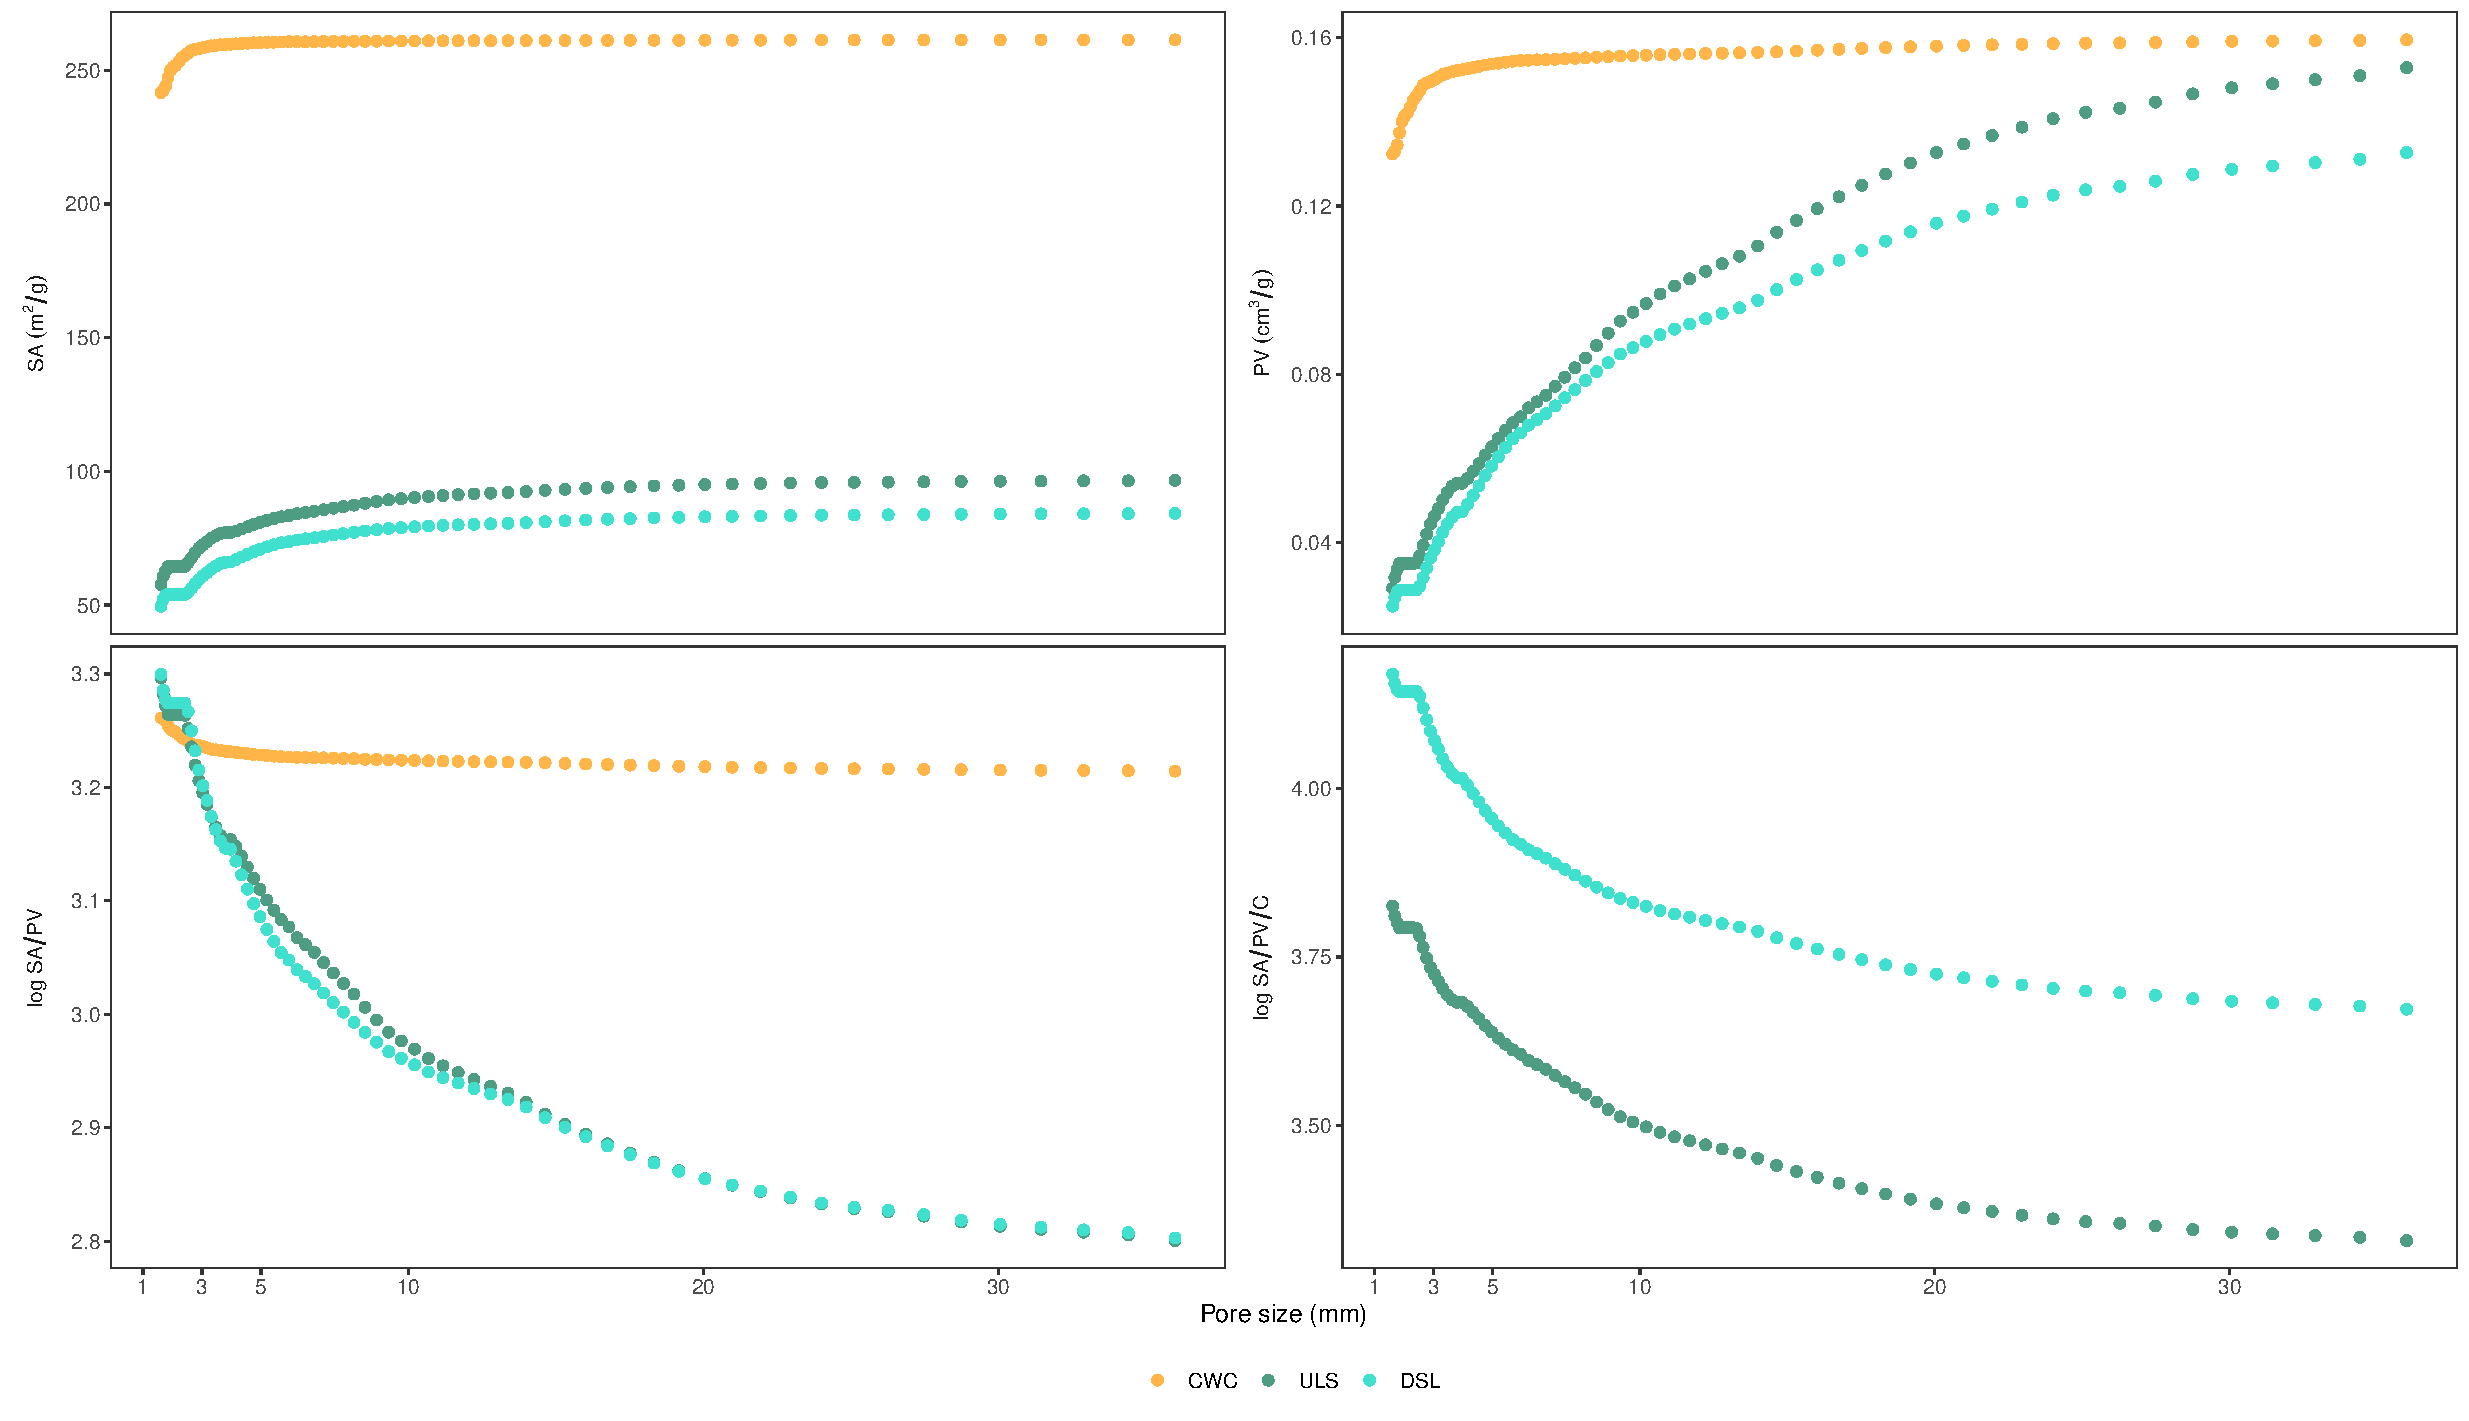
\includegraphics[height=6cm]{R/figs/Kd_1ugL_Fe.pdf}
        \caption{}
        \label{subfig:Fe}
    \end{subfigure}%
    ~ 
    \begin{subfigure}[t]{0.5\textwidth}
        \centering
        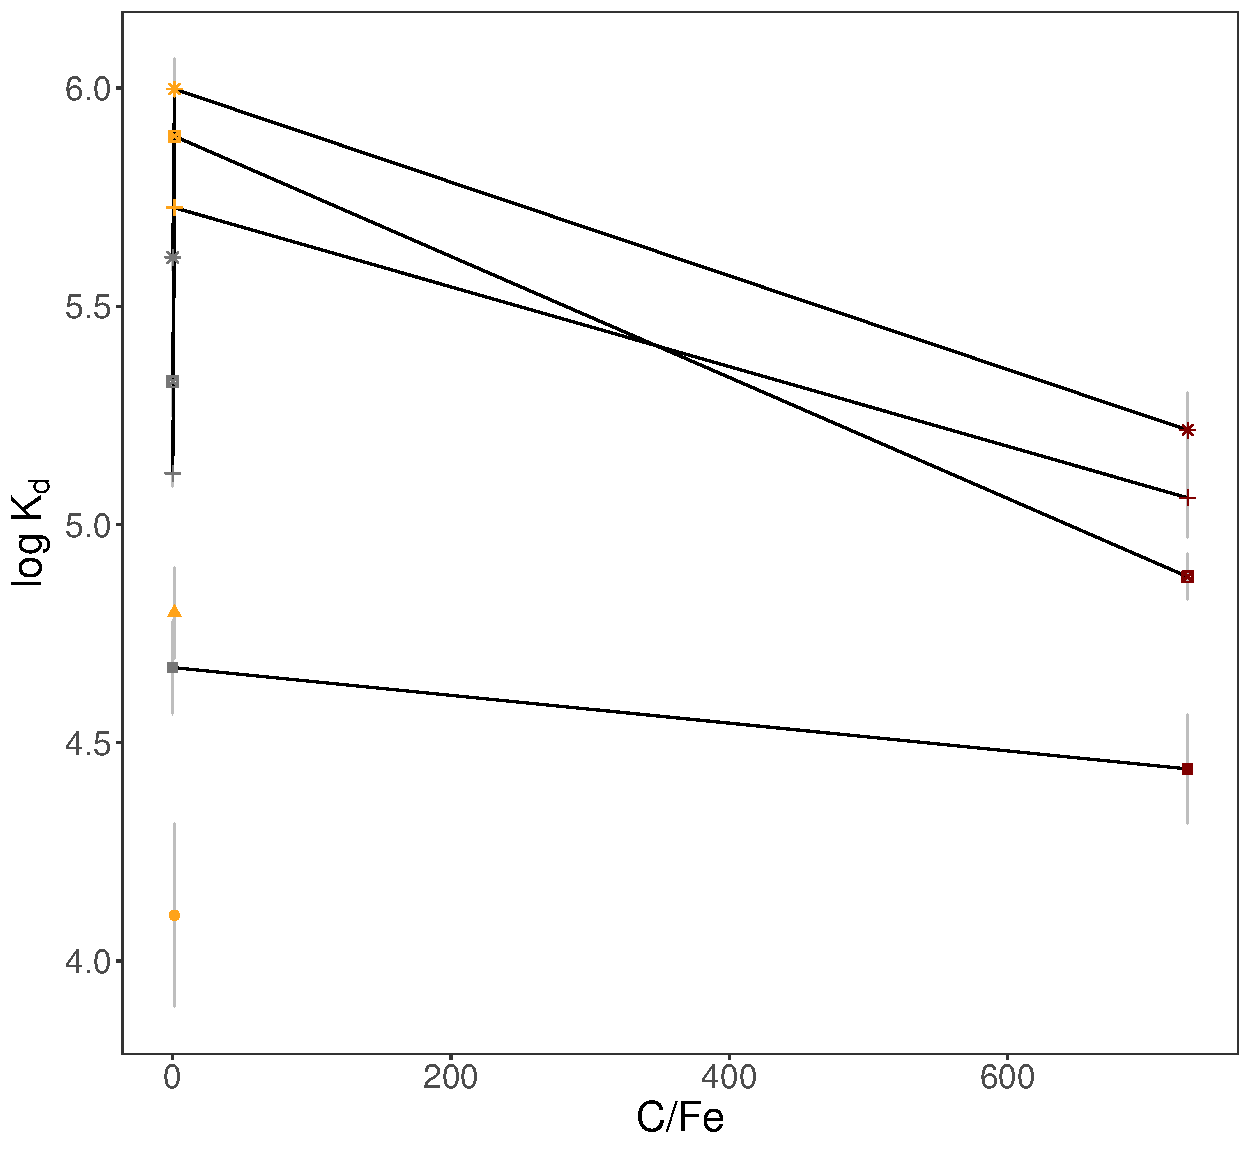
\includegraphics[height=6cm]{R/figs/Kd_1ugL_C_Fe.pdf}
        \caption{}
        \label{subfig:C_Fe}
    \end{subfigure}
    \label{fig:C_Ca_Fe}
    \caption{}
\end{figure*}

\subsubsection{Surface area and pore volume}
Biochar from clean wood chips had a specific surface area (SSA) of 323  m\textsuperscript{2} g\textsuperscript{-1} for large pores (\textgreater 1.5 nm, N\textsubscript{2}), $\sim$ 200 m\textsuperscript{2} g\textsuperscript{-1} higher than the ULS and DSL sludge chars (128 and 110  m\textsuperscript{2} g\textsuperscript{-1}, respectively) \cref{tab:SAPV}. SSA of small pores (0.4-1.5 nm, CO\textsubscript{2} sorption) was 600 m\textsuperscript{2} g\textsuperscript{-1} for CWC, $\sim$ six times higher than ULS and DSL (165 and 87  m\textsuperscript{2} g\textsuperscript{-1}, respectively). Pore volume for large and small pores were relatively similar across biochar types (within 0.1 and 0.15 cm\textsuperscript{3} g\textsuperscript{-1} respectively). Contrary to previous findings, surface area and pore volume does not correlate with higher sorption as CWC proved to be the weakest sorbent in this study. A lack of significant linear correlations between SSA and $K_d$ and PV and K\textsubscript{d} is not surprising due to few biochar samples (n=3). 

Pore size distribution is important for explaining sorption of PFAS of increasing chain lengths due to differences in molecular size. PFDA has a maximum diameter of 1.54 nm, and therefore experiences size exclusion for the smallest pores (0.5-1.5 nm) and can therefore only diffuse into the larger pores represented by N\textsubscript{2} (\textgreater 1.5 nm) (\cref{tab:molecsize}). Regardless of the critical separation at pore size greater/less than 1.5 nm, shorter-chain PFCAs is expected to diffuse more easily into the pores than the larger compounds.  

\citep{Hale2016}: SA and sorption. name variables that showed the strongest correlation with log KF although r2 values were low. Maximum sorption occurs when the molecular dimensions of the PFAS congeners fit inside the pores called size exclusion. Size exclusion is particularly prominent for biochars that are dominated with small micropores, 

PFAS are quite rigid muscularly, so the chains are not flexible to fit into small pores. 

\begin{table}
\centering
\caption{Surface area, pore volume and elemental content (C, O, H, N) and ratios for the biochars produced for the batch tests.}
\adjustbox{max width=\textwidth}{
\label{tab:SAPV}
\begin{tabular}{lllllllllllll}
\toprule
Biochar & Pyrolysis & \multicolumn{2}{l}{N\textsubscript{2} sorption} & \multicolumn{2}{l}{CO\textsubscript{2} sorption} & \multicolumn{4}{c}{Elemental content} & \multicolumn{3}{c}{Elemental ratio} \\
sorbent & temperature & \multicolumn{2}{l}{(pores \textgreater 1.5 nm)} & \multicolumn{2}{l}{(pores 0.4-1.5 nm)} & & & & & & & \\ \cmidrule(l){3-4} \cmidrule(l){5-6} \cmidrule(l){7-10} \cmidrule(l){11-13} & (\textdegree C) & Surface area  & Pore volume & Surface area & Pore volume  & C & O & H & N & O/C & H/C & N/C \\
& & ($\mathrm{m^2~g^{-1}}$) & (cm\textsuperscript{3} g\textsuperscript{-1}) & ($\mathrm{m^2~g^{-1}}$) & (cm\textsuperscript{3} g\textsuperscript{-1}) & (\%) & (\%) & (\%) & (\%) & & & \\ \midrule
CWC & 700 & 323 & 0.017 & 683 & 0.186 & 91.4 & 5.50 & 1.01 & 0.69 & 0.06 & 0.01 & 0.008       \\
ULS & 700 & 128 & 0.126 & 165 & 0.047 & 29.6 & 57.1 & 1.24 & 1.13 & 1.9  & 0.04 & 0.04        \\
DSL & 700 & 110 & 0.111 & 87  & 0.027 & 13.5 & 61.4 & 1.05 & 0.82 & 4.6  & 0.08 & 0.06       \\ \bottomrule
\end{tabular}}
\end{table}


\begin{table}
\caption{Effective cross-sectional diameter (D\textsubscript{eff}) and maximum diameter (D\textsubscript{max}) of TCs interpolated and extrapolated by linear regression from calculations performed by \cite{inoue2012size} on PFOA and other PFCAs with chain lengths 11-18.}
\centering
\begin{threeparttable}
\label{tab:molecsize}
\begin{tabular}{llll}
\toprule
Compound & CF\textsubscript{2} & D\textsubscript{eff} & D\textsubscript{max} \\ 
& chain & (nm) & (nm) \\ \midrule
PFPeA & 5  & 0.45  & 0.96  \\
PFHxA & 6  & 0.50  & 1.08  \\
PFHpA & 7  & 0.56  & 1.19  \\
PFOA\textsuperscript{*} & 8 & 0.61 & 1.36 \\
PFNA & 9 & 0.67 & 1.42  \\
PFDA & 10 & 0.72 & 1.54  \\ \bottomrule                                    
\end{tabular}
\begin{tablenotes}
\item \textsubscript{*} Value from \cite{inoue2012size}
\end{tablenotes}
\end{threeparttable}
\end{table}


\begin{table}
\centering
\caption{Correlation table $log~K_d$ normalized to 1 \textmu g L\textsuperscript{-1} $C_w$.}
\label{tab:correlation}
\adjustbox{max width=\textwidth}{
\begin{tabular}{lrrrrrrrrrrrrrrrrrr} \toprule
PFCA & \multicolumn{2}{c}{Ca} & \multicolumn{2}{c}{Fe} & \multicolumn{2}{c}{C} & \multicolumn{2}{c}{C/Ca} & \multicolumn{2}{c}{C/Fe} & \multicolumn{2}{c}{SA small} & \multicolumn{2}{c}{PV small} & \multicolumn{2}{c}{SA large} & \multicolumn{2}{c}{PV large} \\ \cmidrule(l){2-3} \cmidrule(l){4-5} \cmidrule(l){6-7} \cmidrule(l){8-9} \cmidrule(l){10-11} \cmidrule(l){12-13} \cmidrule(l){14-15} \cmidrule(l){16-17} \cmidrule(l){18-19}
 & \multicolumn{1}{c}{$r^2$} & \multicolumn{1}{c}{$p$} & \multicolumn{1}{c}{$r^2$} & \multicolumn{1}{c}{$p$} & \multicolumn{1}{c}{$r^2$} & \multicolumn{1}{c}{$p$} & \multicolumn{1}{c}{$r^2$} & \multicolumn{1}{c}{$p$} & \multicolumn{1}{c}{$r^2$} & \multicolumn{1}{c}{$p$} & \multicolumn{1}{c}{$r^2$} & \multicolumn{1}{c}{$p$} & \multicolumn{1}{c}{$r^2$} & \multicolumn{1}{c}{$p$} & \multicolumn{1}{c}{$r^2$} & \multicolumn{1}{c}{$p$} & \multicolumn{1}{c}{$r^2$} & \multicolumn{1}{c}{$p$} \\ \midrule
PFPeA & 0.92 & 0.19 & 0.87 & 0.23 & 0.87 & 0.23 & 0.77 & 0.31 & 0.71 & 0.36 & 0.81 & 0.28 & 0.81 & 0.29 & 0.78 & 0.31 & 0.59 & 0.44 \\
PFHxA & 0.1 & 0.79 & 0.1 & 0.79 & 0.15 & 0.74 & 0.25 & 0.66 & 0.32 & 0.62 & 0.21 & 0.69 & 0.22 & 0.69 & 0.25 & 0.67 & 0.44 & 0.54 \\
PFHpA & 0.15 & 0.75 & 0.069 & 0.83 & 0.2 & 0.7 & 0.31 & 0.62 & 0.38 & 0.58 & 0.27 & 0.65 & 0.27 & 0.65 & 0.31 & 0.63 & 0.51 & 0.5 \\
PFOA & 0.1 & 0.79 & 0.11 & 0.79 & 0.15 & 0.74 & 0.25 & 0.67 & 0.32 & 0.62 & 0.21 & 0.7 & 0.22 & 0.69 & 0.25 & 0.67 & 0.44 & 0.54 \\
PFNA & 0.42 & 0.55 & 0.0026 & 0.97 & 0.5 & 0.5 & 0.62 & 0.42 & 0.69 & 0.38 & 0.58 & 0.45 & 0.58 & 0.45 & 0.62 & 0.42 & 0.8 & 0.29 \\
PFDA & 0.5 & 0.5 & 0.015 & 0.92 & 0.57 & 0.45 & 0.69 & 0.38 & 0.75 & 0.33 & 0.65 & 0.41 & 0.65 & 0.4 & 0.69 & 0.38 & 0.86 & 0.25 \\
 &  &  &  &  &  &  &  &  &  &  &  &  &  &  &  &  &  &  \\ \midrule
PFCA & \multicolumn{2}{c}{SA large/Fe} & \multicolumn{2}{c}{SA large/Ca} & \multicolumn{2}{c}{SA small/Fe} & \multicolumn{2}{c}{SA small/Ca} & \multicolumn{2}{c}{PV large/Fe} & \multicolumn{2}{c}{PV large/Ca} & \multicolumn{2}{c}{PV small/Fe} & \multicolumn{2}{c}{PV small/Ca} &  &  \\ \cmidrule(l){2-3} \cmidrule(l){4-5} \cmidrule(l){6-7} \cmidrule(l){8-9} \cmidrule(l){10-11} \cmidrule(l){12-13} \cmidrule(l){14-15} \cmidrule(l){16-17}
 & \multicolumn{1}{c}{$r^2$} & \multicolumn{1}{c}{$p$} & \multicolumn{1}{c}{$r^2$} & \multicolumn{1}{c}{$p$} & \multicolumn{1}{c}{$r^2$} & \multicolumn{1}{c}{$p$} & \multicolumn{1}{c}{$r^2$} & \multicolumn{1}{c}{$p$} & \multicolumn{1}{c}{$r^2$} & \multicolumn{1}{c}{$p$} & \multicolumn{1}{c}{$r^2$} & \multicolumn{1}{c}{$p$} & \multicolumn{1}{c}{$r^2$} & \multicolumn{1}{c}{$p$} & \multicolumn{1}{c}{$r^2$} & \multicolumn{1}{c}{$p$} &  &  \\ \midrule
PFPeA & 0.71 & 0.36 & 0.75 & 0.33 & 0.71 & 0.36 & 0.75 & 0.33 & 0.74 & 0.34 & 0.27 & 0.65 & 0.71 & 0.36 & 0.75 & 0.33 &  &  \\
PFHxA & 0.32 & 0.62 & 0.28 & 0.65 & 0.32 & 0.62 & 0.27 & 0.65 & 0.29 & 0.64 & 0.76 & 0.32 & 0.32 & 0.62 & 0.28 & 0.65 &  &  \\
PFHpA & 0.38 & 0.58 & 0.34 & 0.61 & 0.38 & 0.58 & 0.33 & 0.61 & 0.35 & 0.6 & 0.81 & 0.28 & 0.38 & 0.58 & 0.33 & 0.61 &  &  \\
PFOA & 0.32 & 0.62 & 0.28 & 0.65 & 0.32 & 0.62 & 0.27 & 0.65 & 0.29 & 0.64 & 0.76 & 0.32 & 0.32 & 0.62 & 0.27 & 0.65 &  &  \\
PFNA & 0.69 & 0.38 & 0.65 & 0.41 & 0.69 & 0.38 & 0.65 & 0.41 & 0.66 & 0.4 & 0.98 & 0.082 & 0.69 & 0.38 & 0.65 & 0.41 &  &  \\
PFDA & 0.75 & 0.33 & 0.72 & 0.36 & 0.76 & 0.33 & 0.71 & 0.36 & 0.73 & 0.35 & 1 & 0.035 & 0.76 & 0.33 & 0.71 & 0.36 &  & \\ \bottomrule
\end{tabular}}
\end{table}

\subsubsection{Iron speciation}
Synchrotron results 

\subsubsection{PZC}

\subsubsection{pH and conductivity}
pH varied little between all biochar-soil-water systems with an average pH of 7.18 \textpm 0.02. Conductivity was 39 \textpm 0.9 \textmu S cm\textsuperscript{-1}. Since the variance is low, pH and conductivity was not considered as factors that influence sorption of PFCAs. The conductivity of soil-water samples differed the most from the rest of the samples with a mean conductivity of 23 \textpm 0.05 \textmu S cm\textsuperscript{-1} versus a mean of 41 \textpm 0.9 \textmu S cm\textsuperscript{-1} for the biochar-water and biochar-soil-water samples. Complete pH and conductivity data is in \cref{appSec:misclab}.

\citep{zhang2013sorption}: sorption of PFAS increases with decreasing pH

\begin{table}
\centering
\caption{Mean pH and conductivity (\textmu S cm\textsuperscript{-1}) measurements for the different batch test systems (n=3). The error bars represent the standard error. BC/S/L is the biochar:soil:liquid ratio.}
\label{tab:pHcond}
\begin{tabular}{lccccc}
\toprule
 & \multicolumn{2}{c}{pH} & \multicolumn{2}{c}{Conductivity} & \\ \cline{2-5}
 & mean & std. dev & mean & std. dev & BC/S/L\\ 
\midrule
ULS & 7.10 & 0.04 & 45.70 & 3.03 & 1/0/500\\
DSL & 7.31 & 0.02 & 40.93 & 1.07 & 1/0/500\\
CWC & 7.36 & 0.07 & 46.47 & 0.70 & 1/0/500\\
ULS+S & 7.18 & 0.02 & 34.93 & 0.40 & 1/50/500\\
DSL+S & 7.14 & 0.00 & 35.73 & 1.50 & 1/50/500\\
CWC+S & 7.09 & 0.05 & 44.90 & 1.54 & 1/50/500\\
S & 7.08 & 0.05 & 23.33 & 0.87 & 0/1/10\\
\bottomrule
\end{tabular}
\end{table}

\subsection{Sorption non-linearity}
$n_F$ is a dimensionless empirical parameter that represents sorption linearity, where $n<$ indicates sorption attenuation. All isotherms experience sorption site saturation at increasing concentrations indicated by $n_F<1 $ (\cref{tab:summary_stats_single}, which is consistent with the Freundlich model and other studies where sorption to biochar sees $n$-values typically around 0.3-0.7 \citep{Cornelissen2005}. From other studies, $K_F$ increases and $n_F$ decreases with decreasing O/C, H/C, and N/C ratios \citep{Cornelissen2005}. However, this study $K_F$ decreases with decreasing O/C, H/C, and N/C ratios, and no clear trend is seen for $n_F$ \cref{subfig:n}. Meanwhile, it does seem like the nonlinearity coefficients for CWC are more stable with increasing chain lengths than ULS and DSL. Additionally, comparing $n$ across compound isotherms does not make sense due to different spike concentrations being used for each compound. \citep{yin2022insights} suggests that electrostatic interactions between PFCAs and sediment can contribute to further enhancement of saturation of the adsorption sites and that intermolecular electrostatic repulsion between the individual molecules could also result in nonlinear sorption \citep{higgins2006sorption,yin2022insights}.

\citep{yin2022insights} attributes non-linear sorption to three explanations: 1) complex composition of biochar with negative, positive and neutral charges within same matrix, 2) successive saturation of adsorption sites, 3) electrostatic interactions between the PFASs and sediment, 4) electrostatic repulsion from negatively charged carboxylate groups. 

Sorption non-linearity ($n<1$) occurs due to the complex composition of sediment/biochar with both positive and negative charges contributing to either attraction or repulsion, as well as hydrophobic surfaces, and indicates successive saturation of these adsorption sites \citep{yin2022insights}.  

For the short-chain compounds (PFPeA and PFHxA), Correlations are poor which results in higher standard errors and slopes that are unrealistic (PFHxA-DSL: n=1.11 and PFHpA-ULS: 1.08). Possible explanations for the poor correlations for PFPeA and PFHxA are poor biochar affinity, but the standard error is also large so that the isotherm may actually be linear ($\pm$ 0.11 for both). For PFPeA- and PFHxA-CWC, it appears that CWC sorption sites have been saturated since most points center around the same area, which means that CWC reaches sorption maximum at $~$4000 $\mu g~kg^{-1}$. However, four points are insufficient to conclude that CWC has the lowest affinity and capacity to sorb short-chain PFCAs. The CWC isotherms had the widest concentration intervals for $C_w$, which can be explained by CWC being the weakest sorbent of the three biochars studied, resulting in higher aqueous concentrations than for the sludge biochars. 

\subsubsection{Isotherm concentration range}
The importance of a wide enough concentration interval is reflected in the resulting $n_F$-value acheived. ULS and DSL gave isotherms typically across 0-1.5 orders of magnitude, which indicates that either higher spike concentrations or a lower BC dosage should have been used for the batch tests and that the sludge biochars have a higher sorptive capacity compared with CWC. The batch tests were spiked at 10 concentrations over four orders of magnitude where the lowest concentration was aimed at being close to the instrumental LOQ. Poor signals were achieved for the SC1 points and were removed from the data analysis to improve the certainty of the regression analysis. By doing this the concentration range was reduced. The concentration range achieved was an average of 1.3 log units for the batch test filtrate, in contrast to the desired concentration range over 4 log units.

\section{Sorption attenuation in a PFCA cocktail}
Sorptive attenuation of a spiked cocktail of the six TCs were tested for each biochar is shown by the red point in \cref{fig:sorption_isotherms_all}. Due to different spike concentration used for each compound in the cocktail, establishing quantitative trends for how chain length influences competition for sorption size is difficult. However, some conclusions can be drawn by looking at the overall trends. \cref{tab:competition} shows that $log~K_d$ decreases for all compounds in the presence of a mixture. $K_d$ changes the least for PFHxA and PFHpA (2.3 and 0.2 \% respectively) and may be attributed to lower spiked concentrations (330 and 117 \textmu g L\textsuperscript{-1}) for these compounds compared to the rest in \cref{tab:competition}. Competition is most profound for PFOA to CWC followed by PFDA for ULS and CWC (15.8, 10.0 and 10.6 \% respectively), which can be explained by the highest concentrations spiked for these compounds (1 953 and 3 830 \textmu g L\textsuperscript{-1}). It appears that sorption of PFNA is minimally influenced by competition between other compounds despite SC being in the higher range (1 409 \textmu g L\textsuperscript{-1}). $K_d$ for PFPeA is reduced by 8.2\% and is expected based on weaker sorption of short-chain compounds.

Expected: Attenuation factors larger for short-chain than long chains which have greater sorption affinity.

\begin{figure}
    \centering
    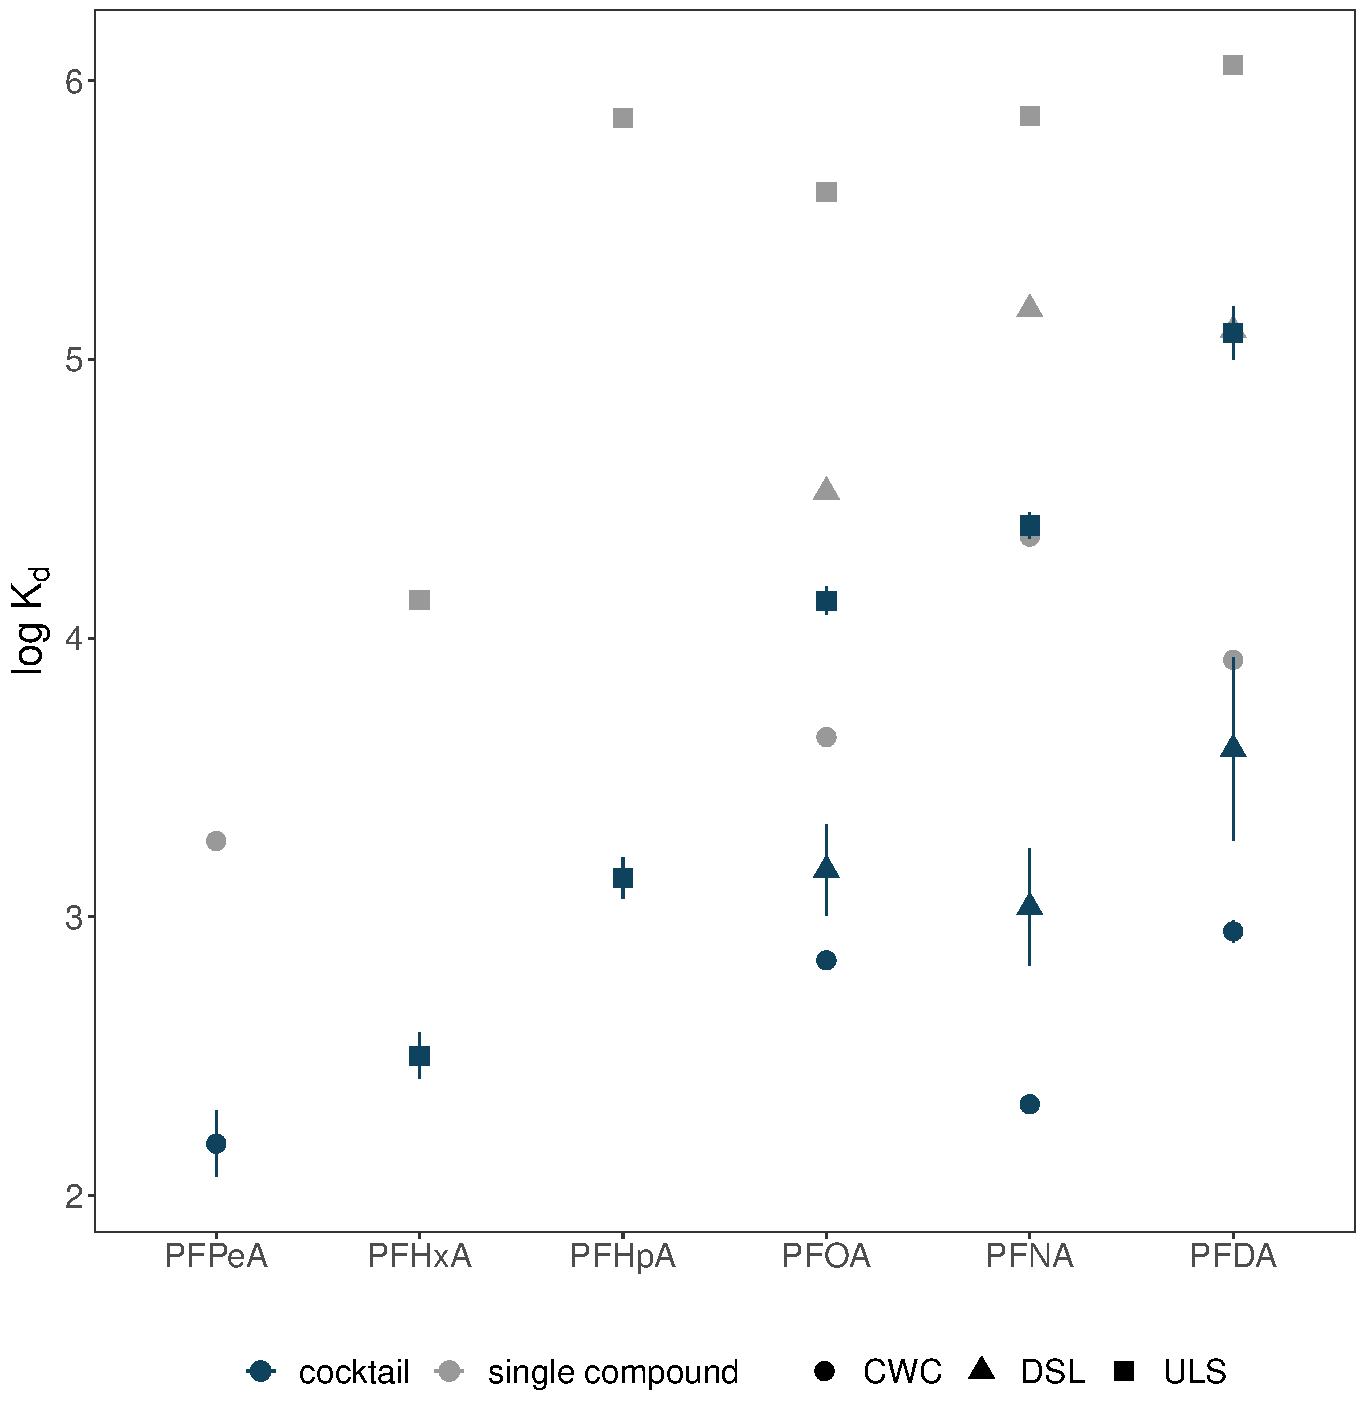
\includegraphics[width=\textwidth]{R/figs/C10_mixVsSingle_BC_plot.pdf}
    \caption{Sorption attenuation for TCs in a cocktail spiked at SC10. It is important to note that attenuation cannot be compared across chain lengths as different concentrations have been used. The error bars represent the standard deviation of $log~K_d$ for the cocktail batch tests performed in triplicate. The single-compound $log~K_d$'s are single points.}
    \label{fig:competition}
\end{figure}

\begin{table}
\centering
\caption{Competition factor at SC10 (\cref{tab:spikeConcentrations}) for each compound and biochar. Competition factor is defined as K\textsubscript{d,single}/K\textsubscript{d,mix})$\times$100\%.}
\begin{threeparttable}
\label{tab:competition}
\begin{tabular}{lrrr}
\toprule
 & \multicolumn{3}{c}{Competition factor \%} \\ \cmidrule(l){2-4}
 & CWC & ULS & DSL \\ \midrule
PFPeA & 8.2 & \textsuperscript{*} & \textsuperscript{*} \\
PFHxA & \textsuperscript{*} & 2.3 & \textsuperscript{*} \\
PFHpA & \textsuperscript{*} & 0.2 & \textsuperscript{*} \\
PFOA & 15.8 & 3.4 & 4.4 \\
PFNA & 0.9 & 3.4 & 0.7 \\
PFDA & 10.6 & 10.9 & 3.1 \\ \bottomrule
\end{tabular}
\begin{tablenotes}
\item \textsuperscript{*} Amount in filtrate exceeded the amount spiked due to analytical uncertainty.
\end{tablenotes}
\end{threeparttable}
\end{table}


%%%%%%%%%%%%%%%%%%%%%%%%%%%%%%%%%%%%%%%%%%%%%%%%%%%%%%%%%%%%%%%%%%%%%%%%%%%%%%%%%%%%%%%%%%%%%%%%%%%%%%%%%%%%%%%%%%%%%
%%%%%%%%%%%%%%%%%%%%%%%%%%%%%%%%%%%%%%%%%%%%%%%%%%%%%%%%%%%%%%%%%%%%%%%%%%%%%%%%%%%%%%%%%%%%%%%%%%%%%%%%%%%%%%%%%%%%%
%%%%%%%%%%%%%%%%%%%%%%%%%%%%%%%%%%%%%%%%%%%%%%%%%%%%%%%%%%%%%%%%%%%%%%%%%%%%%%%%%%%%%%%%%%%%%%%%%%%%%%%%%%%%%%%%%%%%%

\section{PFAS sorption in soil-biochar-water batch tests}
\subsection{Soil chemistry}
The soil used in the batch tests was characterized as a fine sand (0.1 to 0.3 mm) with 1.3 \% TOC (pH 5.38 \textpm 0.02, CEC 2.63 \textpm 0.06 meqv 100 g\textsuperscript{-1}). Total element concentrations and exchangeable ion concentrations are in \cref{appSec:elements}, \cref{apptab:soil}. The soil extraction showed no native target analytes present.  


Table with partitioning coefficients for the biochar sorbents with and without the presence of soil, plus/minus standard error
Kd at C10 for soil alone
How to account for Kd of soil when calculating KF 
    Show how to derive Freundlich equation with respect to soil Kd from original Freundlich equation
    
\subsection{PFOA isotherms vs cocktail isotherms}
to compare with C$_w$ at SP10 for the single compound batch test to determine a competition factor between the other PFCAs in the cocktail to sorption sites on the biochar.

Plot comparing the isotherms of PFOA-BC to PFOA-soil-BC
Discuss influence of presence of soil on PFOA sorption
Significance of C8 chain length taken together with BC properties 

Plot comparing cocktail-BC to cocktail-soil-BC
Effect of presence of soil AND competing congeners
Competitive sorption, attenuation factor

Comparison between sorption of PFOA in cocktail-soil and PFOA in biochar-soil

\subsection{Sorption attenuation by soil}
fouling/pre-loading by NOM
Pore blocking

\subsection{Soil-BC interactions}
Most previous studies have reported a linear increasing trend between log Kd and chain length. However not for PFPeA, \citep{zhang2013sorption}, found in \citep{Sorengard2019}. and \citep{guelfo2013}  these studies are for sorption to organic matter.  Steric hindrance. 

\subsubsection{Difference in color of filtrate between batch tests}
Filter clogging and reduction in filter size, had to exchange filters during filtration, how this may impact results
Aggregation of humic substances upon addition of acetic acid pre-SPE, how this may impact results

Precipitation of a brown fluff was observed when filtered batch tests containing soil was adjusted to pH 3 with 1 M acetic acid

\begin{figure}
    \centering
        \begin{subfigure}[t]{\linewidth}
            \centering
            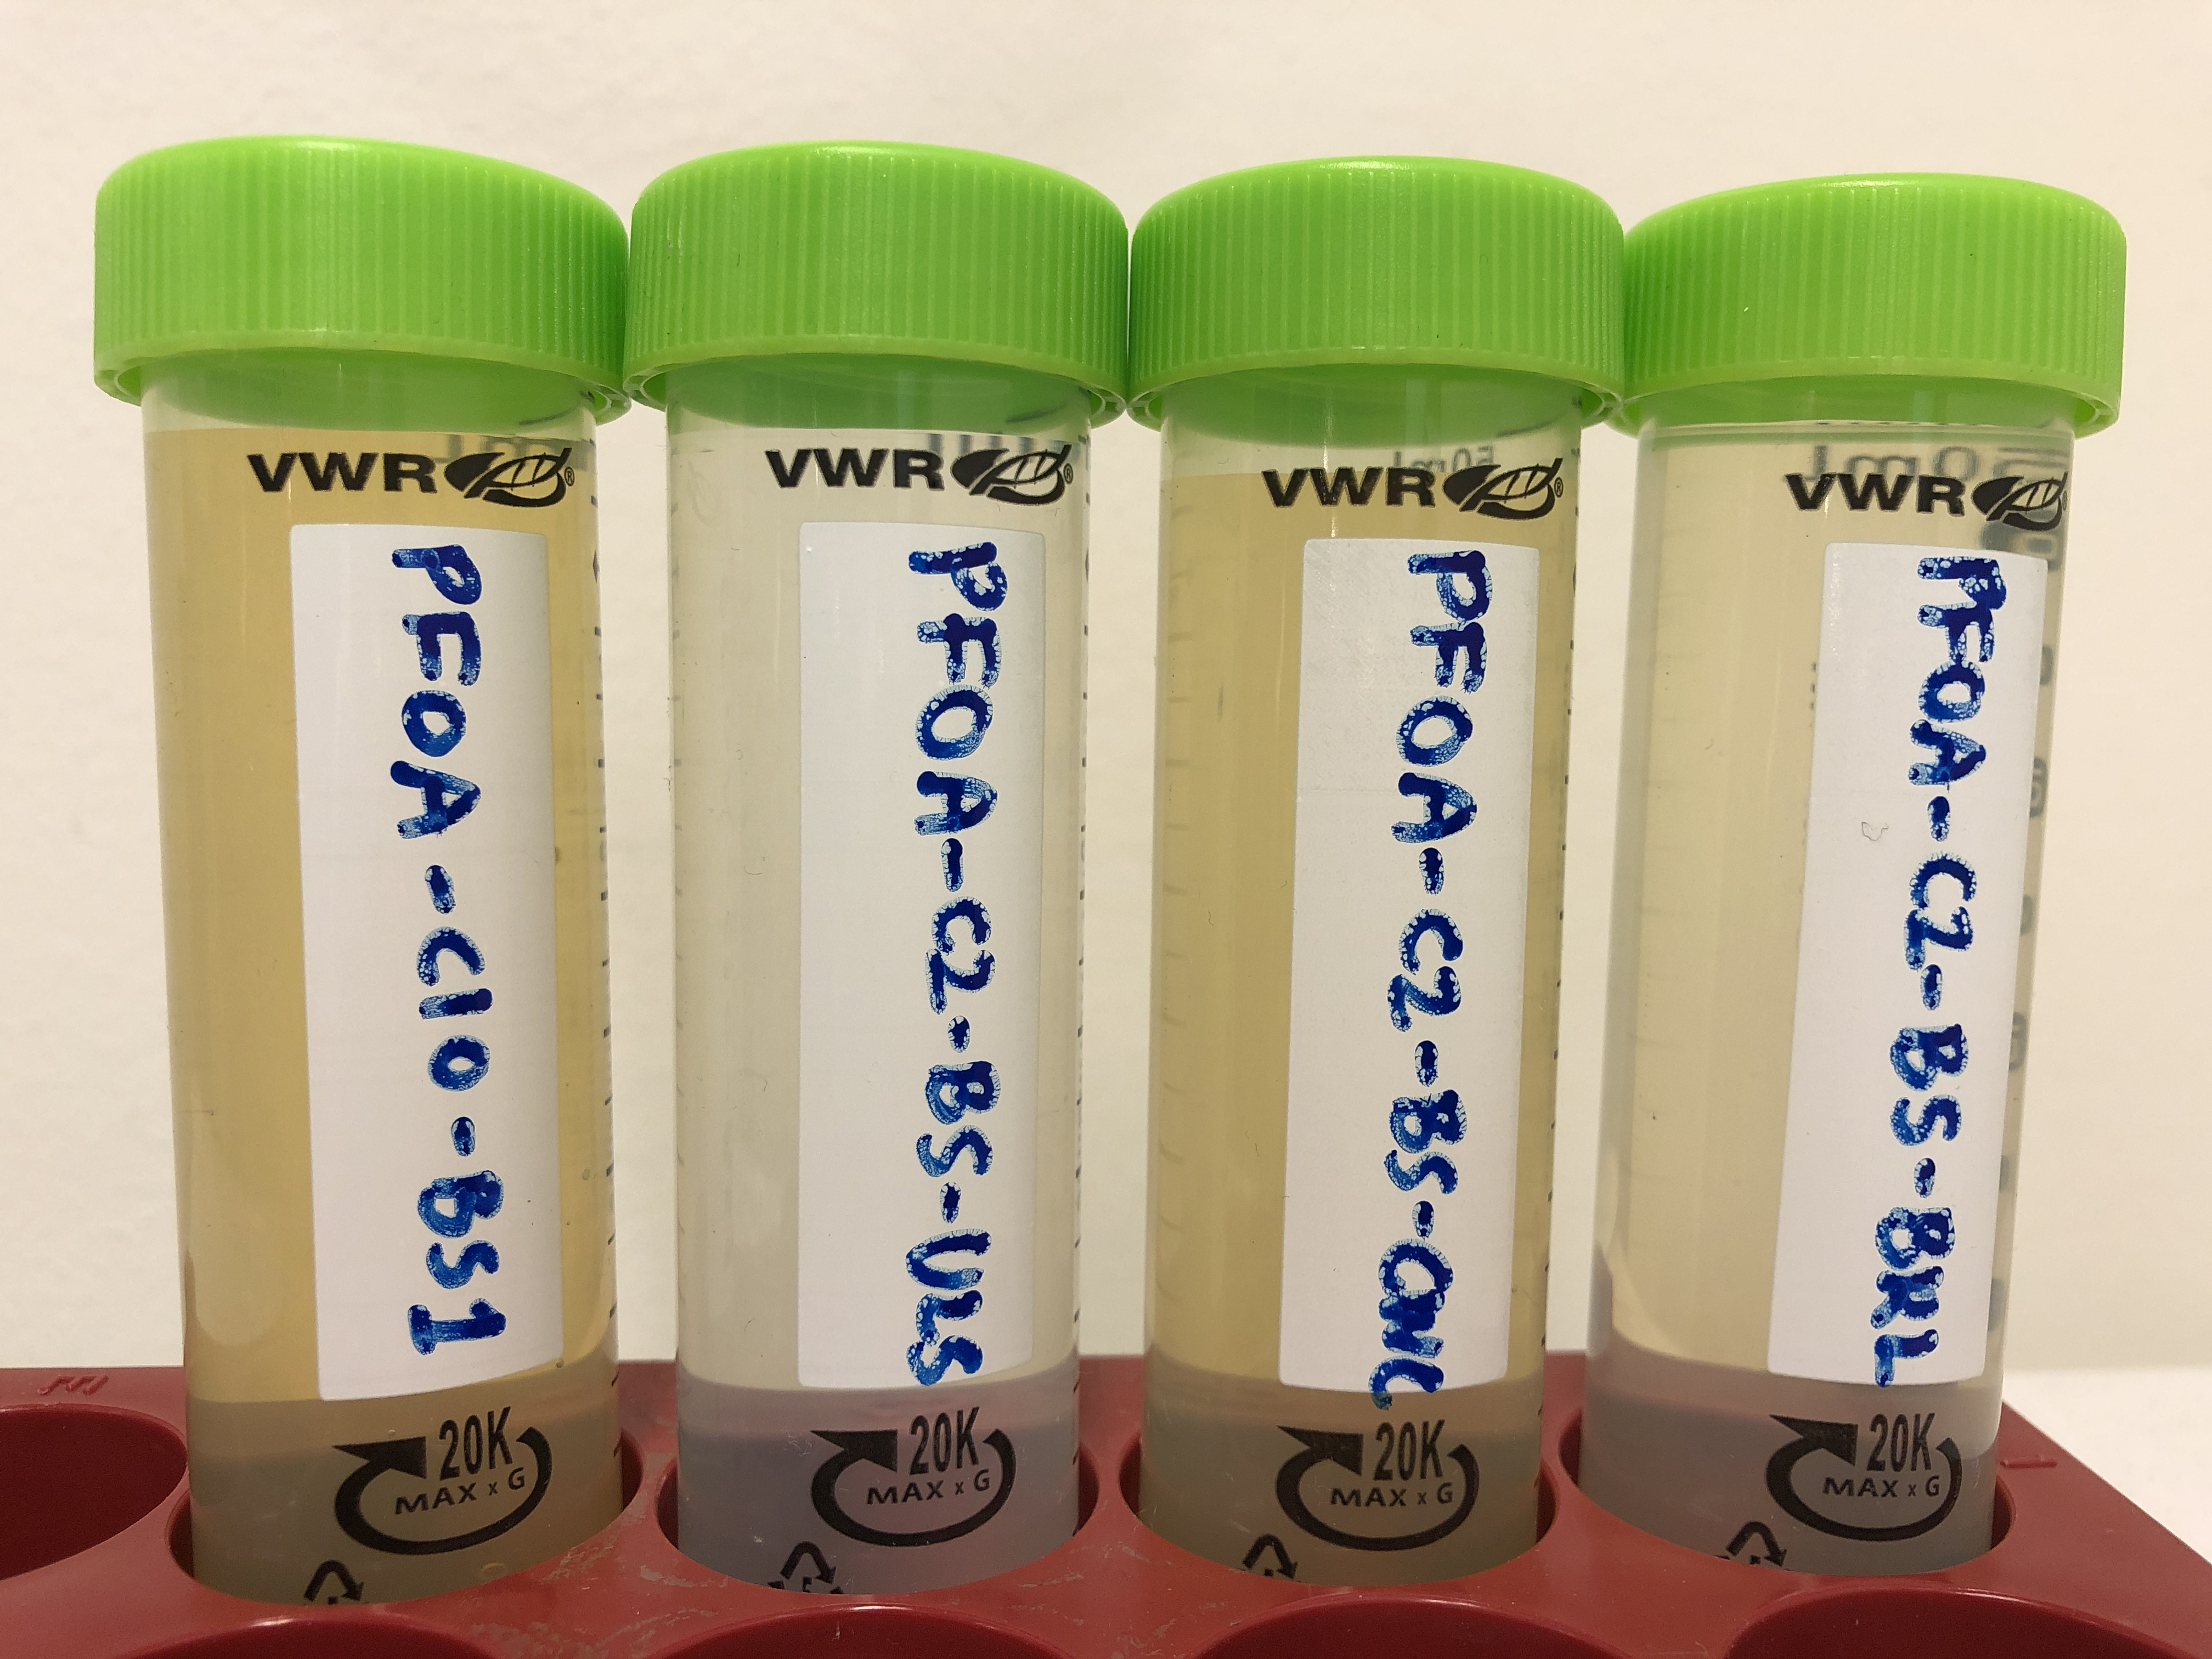
\includegraphics[width=0.6\textwidth]{Bilder/Samples/Filtrate_DOC.JPG}
            \subcaption{}
            \label{fig:filtrate}
        \end{subfigure}
        \begin{subfigure}[]{\linewidth}
            \centering
            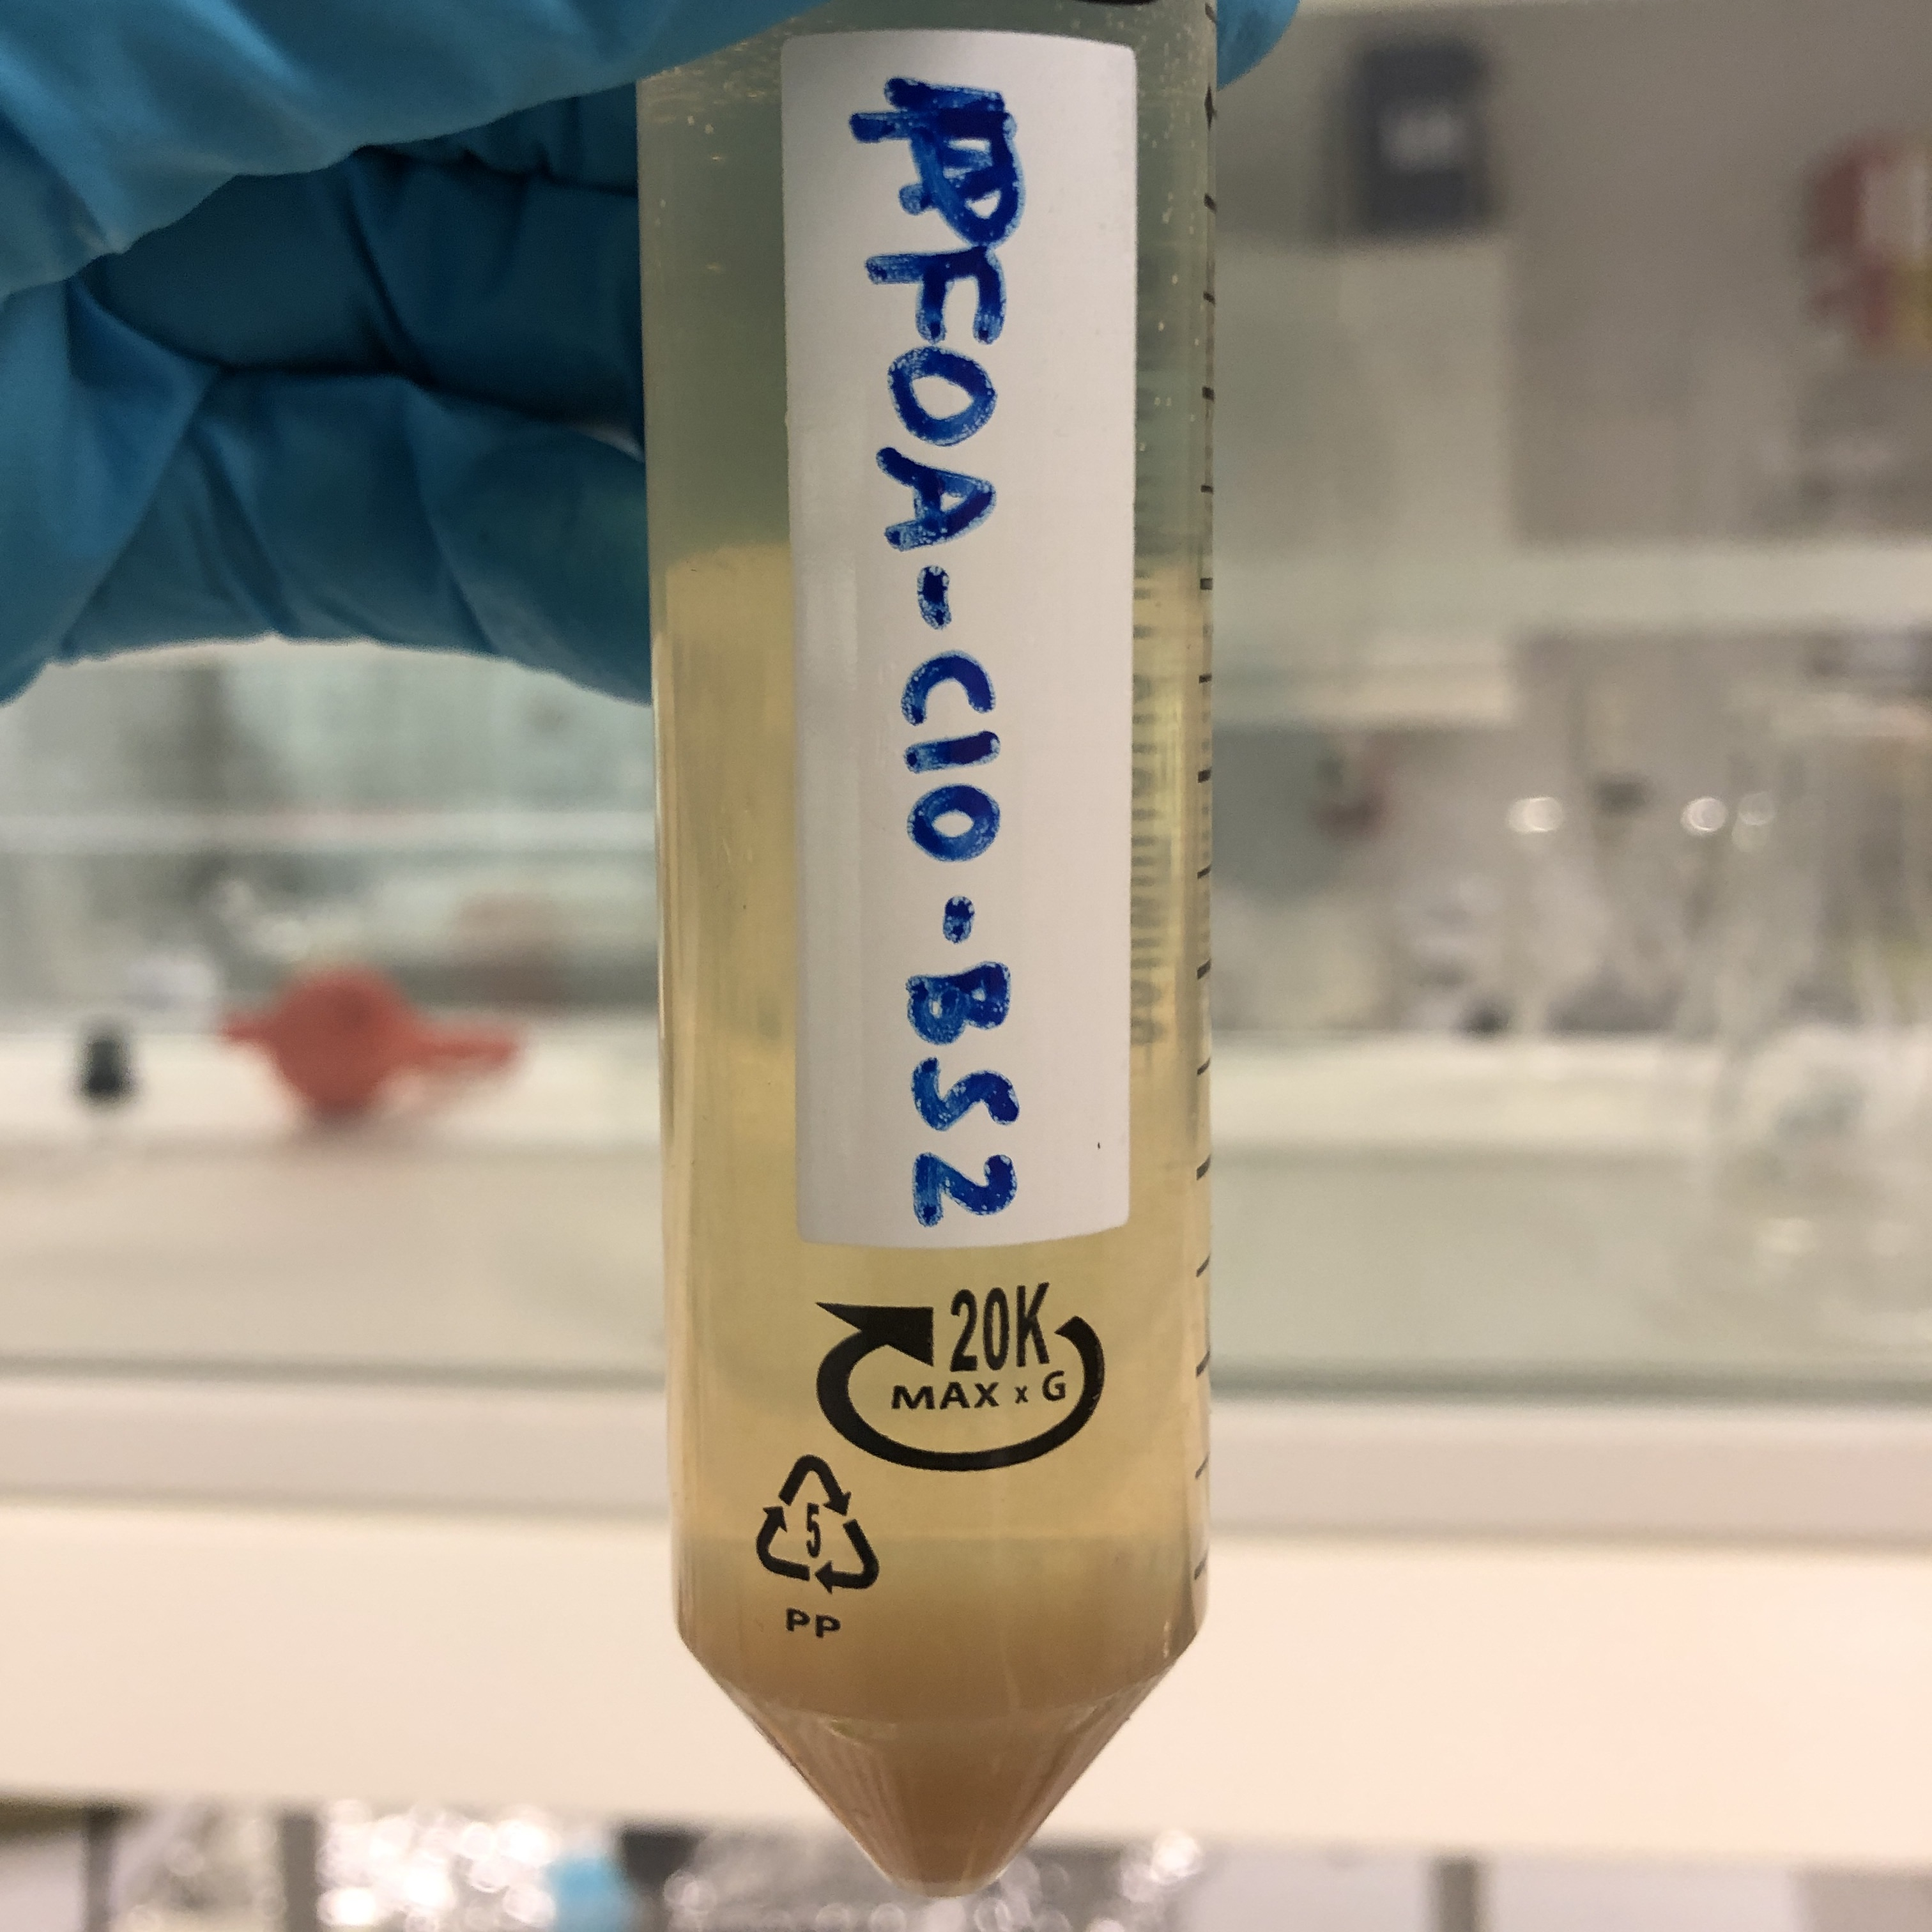
\includegraphics[width=0.6\textwidth]{Bilder/Samples/Precipitation.jpg}
            \subcaption{}
            \label{fig:precip}
        \end{subfigure}  
        \caption{(a) Color of filtrate for each biochar batch test. From left to right: soil only, soil+ULS, soil+CWC, and soil+BRL. (b) Precipitation observed when filtered soil samples were adjusted to pH 3 with 1 M acetic acid.}
        \label{fig:DOC_tubes}
\end{figure}

\section{Potential for commercializing sludge chars as sorbents}
\subsection{Sorbent quality}
Removal efficiency, good enough for application?
\subsubsection{EBC limits heavy metals}
Leaching of heavy metals results at PT 700 C
    As, Cd, Co, Zn, Pb for all chars Below EBC limits, Cr and Ni between lower and upper limit
    EBC = European Biochar Certificate
    Cu above EBC limits for ULS and DSL
    Enrichment factors heavy metals (?)

\subsubsection{Field conditions representativeness}
Soil pH, sorption/desorption of PFAS
Protonation state of PFAS (pKa) unaffected at environmentally relevant pH’s
Leaching in acid soil not a problem, will increase sorption affinity of charged carboxyl to protonated BC surface
Alkaline conditions, liming?? 
    Depends on the dominating sorption mechanism
    Repulsion: functional groups, iron oxides, changes charge with pH?
    If hydrophobic interactions are dominating, sorption will likely not be affected
Equilibrium conditions vs laboratory batch tests
BC dose

Are the results representative of what goes on in real life? Sorption by shaking for 14 days represent an assumed equilibrium between PFCAs in the water and soil phase. A comparable situation in the field would be washing of the soil with large amounts of water such as during heavy rainfall. This will only be the case during occasional stormwater events and thus the results from this research could benefit from being supplemented with results from leaching tests using biochar mixed with soil. However, the relationship:

\begin{align}
    \frac{k_1}{k_2}
\end{align}

where \(k_1\) is the PFCA sorption (adsorption and absorption) rate and \(k_2\) is the PFCA desorption rate, where \(k_1>>k_2\), which indicates that sorption is many times higher, and in an equilibrium situation, sorption and desorption will be at steady state \citep{Cornelissen2005}. 


\section{Sustainability}
\subsection{Pyrolysis energy demand}
\subsection{Life cycle impact assessment (LCIA)}
LCA (life cycle assessment), sustainability aspects of production of biochar
High operating energy and cost different technologies \citep{Alhashimi2017}

\section{Quality control of laboratory analysis and uncertainty}
Standard concentration (but at least leads to underestimation of results)
\subsection{Spiking standard concentrations}
SPE and directly, why?

The pipettes used for making the PFCA dilutions were calibrated. The three pipettes were: 1) 2-10 mL, 2) 200-1000 \textmu L, and 3) 5-50 \textmu L. All pipettes were below the permitted coefficient of variation (CV = 0.3, 0.5, and 2 $\%$ respectively (\cref{appSec:misclab}, \crefrange{appTab:pip2-10}{appTab:pip5-50}).

Since the diameter of the centrifuge tube (30 mm) was larger than that of a volumetric flask and biochar was added prior to the dilution process, the final concentration of the sorbent-sorbate mixture may have a heightened inaccuracy. However, the volume of which 0.1 g biochar occupies can be considered insignificant due to the high absorptive capacity of biochar and small mass used. Therefore a set of 10 centrifuge tubes filled to 50 mL containing 0.1 g CWC were weighed to control the uncertainty of the final dilutions. The results from weighing show that the weight of 10 trials were not accurate but precise, which means that all samples were prepared with the same final volume even though this volume deviates from 50 mL (\cref{appTab:PPcentrifuge}). 

Volume 50 mL weighed vs by eye measurement, diameter of test tube and error
preparation of cocktail standard, not consistent, some individual pipetting. 

\subsubsection{Filter blanks no significant difference}

\subsection{PFAS losses during laboratory analysis}
SPE protocol, many steps, many PP test tubes transfers, saturated PFAS-solutions, internal standard (dilutions had to disregard IS because too low concentration)

\citep{Lath2019labsorb}: 
Syringe filters: sorption of PFOA to centrifuge tubes and filter membranes. Sorption onto syringe surface: negligible due to short residence time (\textless 10 s). 74\% recovery from regenerated cellulose syringe filter. No improvement in recovery was seen when conditioning the syringe filters with phosphate solution or methanol. No trend between losses of PFOA on syringe filter and increasing spike concentrations. Centrifugation only is therefore advised if possible to avoid filtration losses. 

Test tubes: Greater recoveries from glass tubes than plastic, PP poorest recovery (55-68 \% recovery)... Contact time of PFAS residing in tubes for longer than 7 days should not be of significance, as \citep{Lath2019labsorb} propose that sorption and saturation of tube walls occur within hours. 74-81 \% recovery for PP when testing dependence on pH and ionic strength. Slight pH dependence, higher recovery at higher pH due to repulsion of negatively charged functional groups (PP has negative surface charge above pH 3.5-4. Bridging effect will be observed at higher pH's between cations like Ca2+, but is still considered negligible compared to the losses due to the physicochemical properties of the materials themselves. In general PP and plastics consists of mainly carbon hydrogen chains and are more hydrophobic than glassware. Sorption to tube walls saturate, so recoveries increase significantly with higher spike concentrations (e.g. for PP, 12-415 ug/L spiked PFOA increased recovery from 53.7-85.5 \%). Therefore, quantification of low concentrations may be subject to highest error, and in most cases will be an underestimation of dissolved concentrations. 

Use of PP test tubes, study
Higher probability of underestimating Cw for low-concentration samples because tube walls saturate – maximum number of sorption sites, there is a sorption maximum (Langmuir)

\subsection{Uncertainty}
\subsubsection{Batch tests}
Vel, du kan jo prøve å legge sammen alle de feilene. Det finnes jo forskjellige typer feilkilder i et stort forsøksoppsett. Det man ofte ser er at det er en eller to feil som er så store at de overskygger de andre. Da er det ikke noen vits å ta med alle de små. Feilen som ofte er størst er reproduserbarhet av metoden. Altså forskjellen mellom for eksempel prøver laget i triplikater. Det du kan gjøre i oppgaven din er jo å kort diskutere feilkildene du har og identifisere de største og viktigste.

\subsubsection{Analytical}
Calibration curves and matrix effect
LC-MS/MS

\subsubsection{Peak integrations}
Manual review of peak integrations
decisions to remove C1 at low signal
where observed similar peak integrations across concentrations, suspected saturation of detector, dilution of these samples

\subsubsection{Mass balance filters/BC and water}
Why chose only to analyze aqueous phase